% =====================================================================
%  Team Sonar -- Technical, business and pilot report to Mintek
%  (Mintek-SCi Grad Hackathon 2026, Problem 3; Top-5 refinement round)
%  Structure: pitch v8 "three speeds, one decision" -- the belt hyperspectral layer is the site
%  system, the microscope (KHANYA) is the laboratory layer, a person makes the decision.
%  Revision of 7 October 2026 (v7): six-month pilot section, bottom-up pilot budget, TIA structure,
%  TRL milestones, pilot risks; v6 review corrections (Figure 3, labels, fee basis, gate owners).
%  Revision of 6 October 2026 answers an external review: executive summary, decision cadence,
%  bound calibration, throughput-to-value bridge, net-value break-even, exposure by gate,
%  microscope confusion and sensitivity results, held-out disclosure, glossary, appendices.
%  Every internal number traces to a results file in the repository (Appendix D). External facts
%  were re-checked on 5 October 2026; every URL in the reference list was opened on that date.
%  Money is in rand. Planning ranges first set in US$ are converted at R16.4/US$ (FRED EXSFUS,
%  Jan-Sep 2026 monthly mean 16.37).
%
%  BEFORE SUBMITTING: search for "VERIFY". Each one prints in red in the PDF.
%  Compile: tectonic -X compile main.tex   (or pdflatex twice / Overleaf)
% =====================================================================
\documentclass[10pt,a4paper,twocolumn]{article}

\usepackage[a4paper,margin=1.6cm,columnsep=0.6cm]{geometry}
\usepackage[T1]{fontenc}
\usepackage{newtxtext,newtxmath}
\usepackage{microtype}
\usepackage{graphicx}
\usepackage[table]{xcolor}
\usepackage{booktabs,tabularx,array}
\usepackage{enumitem}
\usepackage[font=small,labelfont=bf,skip=4pt]{caption}
\usepackage{tikz}
\usetikzlibrary{arrows.meta,positioning,shapes.geometric,calc}
\usepackage{pgfplots}
\pgfplotsset{compat=1.18}
\usepackage{xurl}
\usepackage[hidelinks]{hyperref}
\urlstyle{same}

\setlist{nosep,leftmargin=*}
\setlength{\parskip}{0pt}
\linespread{0.97}
\raggedbottom
\renewcommand{\topfraction}{0.9}
\renewcommand{\dbltopfraction}{0.97}
\renewcommand{\textfraction}{0.07}
\renewcommand{\floatpagefraction}{0.8}
\renewcommand{\dblfloatpagefraction}{0.8}
\setcounter{topnumber}{3}
\setcounter{dbltopnumber}{4}
\renewcommand{\arraystretch}{1.1}
\newcolumntype{Y}{>{\raggedright\arraybackslash}X}
\newcolumntype{L}[1]{>{\raggedright\arraybackslash}p{#1}}
\newcommand{\backsec}[1]{\par\smallskip\noindent\textbf{#1}\quad\ignorespaces}

\newcommand{\verify}[1]{\textcolor{red}{\textbf{[VERIFY: #1]}}}
\newcommand{\needstech}[1]{\textcolor{orange!85!black}{\textbf{[TECH NUMBERS PENDING: #1]}}}
\newcommand{\cro}{Cr\textsubscript{2}O\textsubscript{3}}
\newcommand{\sha}[1]{\texttt{#1}}
\newcommand{\Wi}{$W_i$}

\definecolor{accent}{RGB}{31,111,178}
\definecolor{copper}{RGB}{180,83,42}
\definecolor{soft}{RGB}{110,110,110}
\definecolor{okgreen}{RGB}{46,125,50}

\title{\vspace{-1.6em}\textbf{REEFPRINT/KHANYA: ore-hardness prediction on the belt and sulphide characterisation in the laboratory.\\ An analogue-data proof of concept and staged validation plan for South African concentrators}\\[3pt]
\large Mintek--SCi Grad Hackathon 2026 \textperiodcentered{} Problem 3: Computer vision for real-time mineralogical characterisation}
\author{Team Sonar: Lethabo Hoaeane\textsuperscript{a}, Sibusiso Khumalo\textsuperscript{b}\\[1pt]
\small \textsuperscript{a}University of South Africa \quad \textsuperscript{b}University of the Witwatersrand}
\date{\small October 2026}

\begin{document}

\twocolumn[
\begin{@twocolumnfalse}
\maketitle
\vspace{-1.8em}
\begin{abstract}
\noindent South African concentrators set mill feed, grind and reagents before the laboratory can say what was in the ore. REEFPRINT/KHANYA combines a working microscope-image workflow with a separate hyperspectral hardness research track, and passes both to an operator who reviews every proposed change. All results so far come from public analogue datasets and a plant simulator. On 146 public porphyry-ore composites the hardness model reached an out-of-fold $R^2$ of 0.479 (colour alone 0.210), its nominal 90\% upper bound covered 93.2\% of samples, and a simulated feed-rate replay estimated a 1.7--1.9\% throughput gain over a fixed design-feed policy. The historically evaluated microscope checkpoint reached IoU 0.870, 0.576 and 0.547 for pyrrhotite, chalcopyrite and pentlandite on 12 sections reused during development; the checkpoint in the audited application build differs, and an independent audit run on one section found large phase-abundance errors. Independent QEMSCAN agreement on unseen South African specimens, and a $\leq$10\% phase-abundance error, are validation targets, not results. We propose a six-month pilot at one host concentrator, costed from the bottom up at R5.27\,million (team, site, reference laboratory and sensor access, with 15\% contingency) and funded mainly through the Technology Innovation Agency (TIA). Its targets are a phase-abundance error of $\leq$10\% on at least 90\% of 30 locked host specimens, and a hardness bound that transfers to host ore. If its gates pass, it takes the microscope from technology readiness level (TRL) 4 to 5--6 and the belt model from TRL~3 to 4--5. Belt capital (US\$250,000--400,000, about R4.1--6.6\,million) follows only after separate transfer gates. As of 7 October 2026, no frozen model has been tested on independent host specimens.
\end{abstract}
\vspace{0.6em}
\vspace{0.3em}
\end{@twocolumnfalse}
]

% =====================================================================
\section{Introduction}

As Team Sonar, working on Mintek's Problem 3, our responsibility is to give a concentrator's shift team a reliable reading of its ore before that ore reaches the mill, and to turn the reading into a plant setting that a person can approve. This report sets out what we built, how we tested it, what it would cost and earn, and, centrally, the six-month pilot that would test it on South African ore (Section~\ref{sec:pilot}). It describes a research prototype: the results are on public analogue data and a simulated plant. It is written for metallurgists, mineralogists, process engineers and the people who fund their technology. Technical terms are defined in the glossary (Table~\ref{app:glossary}).

\subsection{Problem statement}

The brief states the problem plainly: ``without real-time feedback, processing plants cannot adjust to changes in ore quality, leading to inefficient chemical usage and lower mineral yields'' \cite{brief}. Ore reaches the mill within minutes of leaving the belt, whereas assays and automated mineralogy are batch laboratory work. Mintek's own Minerals Processing and Characterisation Cluster runs QEMSCAN automated mineralogy \cite{moodley2026}, and a commercial laboratory describes mineralogy as ``not an overnight assay service'' \cite{als}. Consequently, each shift sets the mill and the flotation circuit for ore whose mineralogy it has not yet seen.


The cost of deciding blind falls most heavily on South Africa, which mined an estimated 120 of the world's 170 tonnes of platinum in 2025 (about 71\%) and 70 of 190 tonnes of palladium. It also holds 63,000 of the world's more than 76,000 tonnes of PGM reserves, mostly in the Bushveld Complex \cite{usgs2026}. The same source attributes the 9\% fall in South African PGM output in 2025 to lower palladium prices, higher deep-level mining costs and disruptions to the electricity supply.

Recovery is where the money is. UG2 ore carries about 30\% \cro{} against about 0.1\% for Merensky ore, and the smelter caps the chromite in concentrate. Mintek testwork made UG2 concentrate at 87\% recovery with 2.9\% \cro{}, and recoveries above 90\% were possible only if the \cro{} limit was relaxed \cite{jones2005}. Producers report recovery moves of this size to investors: Valterra raised concentrator recoveries by 1.2--1.7 percentage points at Mototolo and Amandelbult in 2025 \cite{valterra2025}. Comminution, which sets both liberation and mill throughput, used 52\% of site electricity in a benchmark of mines \cite{ballantyne2012}. Plants do not decide entirely blind: operators, advanced process control (APC) and the mine plan already carry information about the ore. Thus, the decision we aim to improve is narrower: setting mill feed for each parcel of ore before it arrives, with a stated uncertainty, at a cost a producer can recover.

\subsection{Our solution: three speeds, one decision}

REEFPRINT/KHANYA reads the ore at three speeds (Section~\ref{sec:arch}):
\begin{enumerate}
\item \textbf{the belt} (REEFPRINT), every 30 seconds: a short-wave infrared (SWIR) camera above the mill-feed conveyor feeds a model that predicts each parcel's grinding hardness with an upper bound, and Bond's law turns the bound into a mill feed-rate proposal. The belt layer estimates hardness, not mineral identity;
\item \textbf{the laboratory} (KHANYA), once a shift: a microscope model classifies sulphide minerals in polished sections, which addresses the brief's three-phase requirement on slower, prepared samples;
\item \textbf{the decision}: an operator reviews each proposed change before the ore reaches the mill; the site's existing control system keeps authority, and every step is signed and recorded.
\end{enumerate}
It is important to note what is not claimed: real-time mineralogy on the belt, performance on South African ore, a measured plant benefit, or identification of chromite and the silicates. Table~\ref{tab:map} maps the brief and the judging criteria published in the hackathon FAQ (2025 edition; we have not seen a 2026 rubric) \cite{faq} to the evidence, with the status of each.

\begin{table}[t]
\centering\footnotesize
\caption{The brief and the judging criteria: evidence and status. Shown = on public analogue data; Partial = part shown; Proposed = future work; Target = defined, not tested.}
\label{tab:map}
\begin{tabularx}{\columnwidth}{@{}L{1.85cm}YL{1.0cm}@{}}
\toprule
Requirement & Evidence (section) & Status \\
\midrule
$\geq$\,3 mineral phases & Pyrrhotite, chalcopyrite, pentlandite on analogue micrographs (\ref{sec:micro}) & Shown \\
Accuracy report & Belt $R^2$, bound coverage, baselines; microscope results per checkpoint (\ref{sec:belt}--\ref{sec:grains}) & Partial \\
$\leq$\,10\% error & Phase-abundance target defined; not yet tested on independent specimens (\ref{sec:protocol}) & Target \\
Adjust a plant parameter & Feed-rate proposal (designed); regrind advice to a simulator over OPC~UA (\ref{sec:decision}) & Partial \\
Real time & Hardness: 92\,ms per parcel. Mineralogy: laboratory cadence, not on the belt & Partial \\
Local validation & Six-month pilot on host specimens and ore (\ref{sec:pilot}) & Proposed \\
\midrule
Innovation & Bounded hardness input that abstains, with operator review (\ref{sec:methods}) & Shown \\
Feasibility & Pilot plan, team, costs, TIA route, risks, TRL (\ref{sec:pilot}--\ref{sec:roadmap}) & Proposed \\
Impact & Scenario value per 1\% more metal (\ref{sec:finance}) & Scenario \\
Technical execution & Out-of-fold tests, baselines, failed ideas reported; 516 software tests (\ref{sec:results}) & Shown \\
\bottomrule
\end{tabularx}
\end{table}

% =====================================================================
\section{How the system works}\label{sec:methods}

\subsection{Data}

No South African belt scans or labelled Bushveld micrographs were available, so every model was trained and tested on public data (Table~\ref{tab:data}). HIDSAG supplies hyperspectral scans of Chilean porphyry copper--molybdenum drill core with laboratory Bond work-index values \cite{ehrenfeld2023}. LumenStone~S2, a Norilsk nickel--copper sulphide ore \cite{korshunov2025}, shares the mineral assemblage of Bushveld ores but not their abundance: sulphides cover 62.8\% of its sections by area, whereas Merensky ore contains up to about 3\% base-metal sulphides and UG2 less \cite{jones2005}. It supplies labels for the relevant phases, because the base-metal sulphides in UG2 are predominantly pentlandite, chalcopyrite, pyrrhotite and pyrite \cite{jones2005}; its much richer sulphide content and different preparation can still cause transfer failure, which only host specimens can test.

\begin{table}[t]
\centering\footnotesize
\caption{Datasets. All are public; none was supplied by Mintek or a producer.}
\label{tab:data}
\begin{tabularx}{\columnwidth}{@{}L{1.75cm}L{1.55cm}YL{0.95cm}@{}}
\toprule
Dataset & Ore & Size and use & Licence \\
\midrule
HIDSAG \cite{ehrenfeld2023} & Porphyry Cu--Mo, Chile & 146 drill-core composites with Bond work index; visible (39 bands) and SWIR (75 bands). Hardness model & CC0 \\
LumenStone S2 \cite{korshunov2025} & Ni--Cu sulphide, Norilsk & 49 micrographs: 37 train, 12 publisher test (reused in development). Microscope phases & Research use \\
Bushveld assays \cite{bachmann2019} & Bushveld chromitites & 1,112 intervals. Check on PGE routing & CC BY 4.0 \\
\bottomrule
\end{tabularx}
\end{table}

\subsection{The belt layer: hardness from the infrared}\label{sec:beltmethod}

\emph{Sensor (design).} The design uses a SWIR line scanner such as the Specim SX25 (960--2500\,nm, 640 pixels across; 162 lines a second assumed, to be confirmed for the configured unit) with a visible--near-infrared (VNIR) companion camera \cite{specim}. On a 1.2\,m belt moving at 2\,m/s it records a line every 12.3\,mm with 1.88\,mm pixels. It therefore measures parcels of ore, not individual particles. In the pilot design a \emph{parcel} is 30\,s of belt (about 60\,m, or 4,860 scan lines averaged into one spectrum); in the replay reported here, a parcel is one HIDSAG composite scan of 80$\times$117 pixels.

\emph{Model.} Each parcel's spectrum is reduced to features from the infrared absorption regions of clay, mica, chlorite and carbonate minerals (Fig.~\ref{fig:hsi}), and a model predicts the Bond work index (\Wi{}, kWh/t). Results are reported only for samples the model never saw (out of fold), and a result counted only if it beat simple baselines under pass marks committed to the repository before each run. Five targets and several model variants were examined and only the work index survived, so the result is exploratory selection, not a confirmatory test; HIDSAG has no drill-hole identifiers, so grouped independence of the folds cannot be verified.

\emph{Bound and gate.} The plant setting uses an upper bound that the true hardness should stay below 9 times out of 10 (a one-sided 90\% split-conformal bound \cite{lei2018}), not the best guess. A more data-efficient bound \cite{barber2021} was tried first and failed its pass mark, so the exact bound that the plan named as its fallback is used, and the result is provisional. The 90\% is a marginal coverage target that assumes new parcels resemble the calibration data; it is not a per-parcel guarantee and does not certify protection against overload. An out-of-distribution (OOD) check flags parcels unlike anything in training, and their advice is withdrawn.

\subsection{The decision layer and its cadence}\label{sec:decision}

The decision layer turns the hardness bound into a mill setting that a person can approve. Ball mills are usually limited by motor power, so the tonnes a mill can grind depend on how hard the ore is. Bond's law gives the specific grinding energy \cite{bond1961}
\begin{equation}
W = 10\,W_i\left(\frac{1}{\sqrt{P_{80}}}-\frac{1}{\sqrt{F_{80}}}\right)\ \text{kWh/t},
\end{equation}
where $F_{80}$ and $P_{80}$ are the feed and product sizes (\textmu m) passed by 80\% of the material. At a fixed grind target the feed rate the mill can carry is proportional to $1/W_i$, so the proposal is
\begin{equation}
F_{\text{proposed}} = F_{\text{design}} \times \frac{W_{i,\text{design}}}{W_{i,\text{bound}}}.
\end{equation}
The ratio removes explicit power and size terms only when power, feed size, product target and circuit efficiency are held constant; the pilot must test that approximation for the selected circuit. For example, a design hardness of 16.6\,kWh/t and a bound of 16.9\,kWh/t give 98.2\% of design feed, inside an envelope set by the site's metallurgist (85--110\% in the demonstration). The demonstration falls back to 100\% of design feed; at a site, the fallback is the host's own operating procedure.


In the proposed cadence a person approves changes, not every computation: a parcel is scored as soon as it is scanned, and the operator has the rest of an assumed 90\,s belt-to-mill transit to act. A proposal is computed every 30\,s (at most 120 an hour), but the operator sees it only when it differs from the running setpoint by more than a deadband set by the metallurgist (for example 2\% of design feed), and may approve, modify within the envelope, reject or escalate. With no approval in time, a flagged parcel or stale data, the advice is withdrawn and the site's own control policy continues; the system never raises feed on its own. Feed may be cut by up to 10\% but raised by only 3\% per parcel, and the shadow phase measures the real operator-facing rate before anyone acts. Every event is written to a hash-chained record with conventional (Ed25519) and post-quantum (ML-DSA-65 \cite{fips204}) signatures; this supports traceability, not the correctness of the measurement. The microscope's advice reaches a simulated regrind setting over OPC~UA \cite{opcua} (simulated); the feed-rate path is designed, not built.

\subsection{The laboratory layer: minerals under the microscope}\label{sec:micromethod}

The microscope model is a standard image-segmentation network (DeepLabV3 with a ResNet-50 backbone \cite{chen2017,he2016}) that labels every pixel of a reflected-light image as resin, pyrrhotite, chalcopyrite, pentlandite or magnetite. Only the research-approved, historically evaluated checkpoint (SHA-256 \sha{de7135a9}; full hash in Appendix~\ref{app:repro}) may send advice to the simulator. A \emph{Quick} scan classifies six 512-pixel fields of a section; a \emph{full} scan covers the whole section.

Connected regions of the mask are split into grains. For this demonstration, chalcopyrite and pentlandite are treated as payload and pyrrhotite as reject; that assignment is a demonstration assumption for this ore, because pyrrhotite's value depends on PGM deportment and the host's treatment objectives. A grain whose area is at least half payload is \emph{payload-dominant} (shown as ``free'' in the application), otherwise \emph{reject-dominant} (``locked''). This is a 2D payload-area proxy, not a measure of liberation or recoverability; the 50\% line is a declared demonstration choice. A rule-based advisor turns these measures into \emph{grind finer}, \emph{continue}, \emph{verify before acting} or, when the rejected phase dominates, \emph{adjust reagent}. Each is a hypothesis for a metallurgist to test, not an instruction. It answers \emph{verify} when the payload-area estimate lies within $\pm$0.335 of the 50\% line, and gives no recommendation with fewer than 9 payload-bearing grains or mean confidence below 0.85. The $\pm$0.335 band was calibrated on the 12 evaluation sections (Section~\ref{sec:grains}); the other thresholds are placeholders for site metallurgists to set.

\subsection{How we tested it}\label{sec:testing}

Belt models were scored out of fold against the strongest simple baseline (the fold mean, the fold median and a colour-only model), with pass marks committed to the repository before each run. The microscope was scored on the publisher's 12 S2 test sections. They were excluded from network training but reused during development, to compare pipelines, select the checkpoint and calibrate the advisor band, so we report them as \emph{development-influenced evaluation sections}, not an independent test. An independent, source-disjoint local test set is the first deliverable of the laboratory study. Accuracy is the intersection over union (IoU: the overlap between predicted and expert-labelled areas, from 0 to 1), pooled over 103.8 million pixels and averaged per section, with bootstrap confidence intervals over sections. Pixels are correlated within a section, so sections, not pixels, are the independent units. Decision-level agreement runs the same advisor on the model's mask and on the expert's mask; a disagreement is \emph{unsafe} if the model gives a confident instruction that the expert mask does not support. This measures sensitivity to segmentation error, not whether the rules themselves are metallurgically right.

\subsection{Validation targets and independent protocol (proposed)}\label{sec:protocol}

The $\leq$10\% error target must be defined before samples are collected, because absolute and relative errors differ: a reference of 2\,wt\% predicted as 3\,wt\% is a 1-point absolute error but a 50\% relative error. We propose that the mineralogist and a statistician sign an acceptance contract naming the decision-critical phases, an absolute tolerance below an agreed quantification limit and a $\leq$10\% relative target above it, and whether the target applies per specimen or as a phase-wise mean. Microscope image fractions are 2D areas, whereas QEMSCAN modal results are usually mass fractions, and a density conversion alone does not make a polished surface represent bulk mass. The comparison unit, resin exclusion, field selection, section-to-specimen aggregation and density assumptions are therefore fixed in advance; a registered same-surface area-to-area comparison comes first, and bulk mass estimates are validated separately.

A blind test needs more than hiding answers: a separate custodian holds specimen identities and laboratory results; the frozen model receives only acquisition inputs and permitted metadata; predictions are hashed before the reference is revealed; splits are grouped by specimen and collection event; and every refusal stays in the denominator. As a starting envelope we propose 30 development, 10 calibration and at least 30 locked evaluation specimens, subject to a power calculation and laboratory quotes. Zero failures in 30 independent specimens bounds the failure rate at about 9.5\% (one-sided 95\%), which is a statement about pass/fail, not a guarantee of 10\% numerical error. If a model fails, it is fixed on development material and must face a new untouched cohort. As of 7 October 2026 this protocol is drafted, not signed; Section~\ref{sec:goals} gives the pilot's proposed targets.

% =====================================================================
\section{System architecture}\label{sec:arch}

\begin{figure*}[t]
\centering
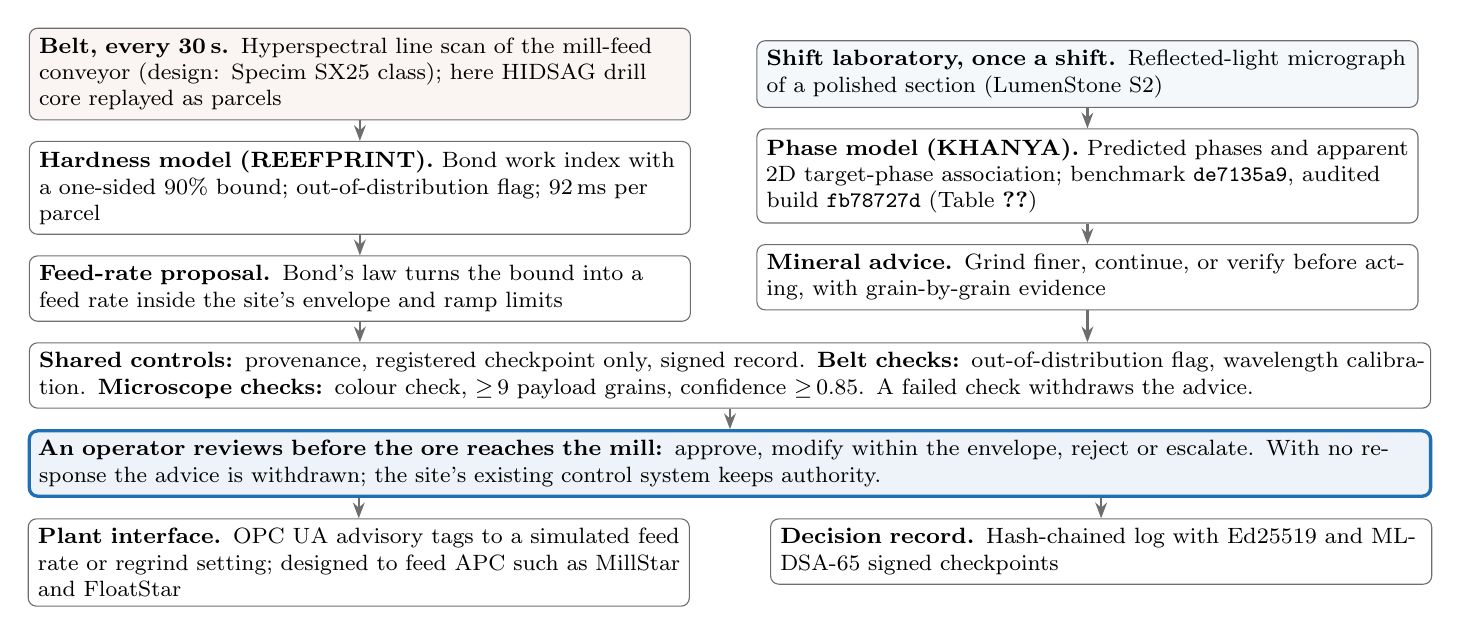
\begin{tikzpicture}[
  box/.style={draw=soft, rounded corners=3pt, align=left, text width=8.15cm, font=\footnotesize, inner sep=3.5pt, minimum height=0.8cm},
  wide/.style={draw=soft, rounded corners=3pt, align=left, text width=17.55cm, font=\footnotesize, inner sep=3.5pt},
  hot/.style={draw=accent, very thick, fill=accent!8, rounded corners=3pt, align=left, text width=17.55cm, font=\footnotesize, inner sep=3.5pt},
  arr/.style={-{Stealth[length=2mm]}, soft, thick}]
\node[box, fill=copper!6] (in1) at (-4.62,0) {\textbf{Belt, every 30\,s.} Hyperspectral line scan of the mill-feed conveyor (design: Specim SX25 class); here HIDSAG drill core replayed as parcels};
\node[box, fill=accent!5] (in2) at (4.62,0) {\textbf{Shift laboratory, once a shift.} Reflected-light micrograph of a polished section (LumenStone S2)};
\node[box, below=0.26cm of in1] (hard) {\textbf{Hardness model (REEFPRINT).} Bond work index with a one-sided 90\% bound; out-of-distribution flag; 92\,ms per parcel};
\node[box, below=0.26cm of in2] (seg) {\textbf{Phase model (KHANYA).} Predicted phases and apparent 2D target-phase association; benchmark \sha{de7135a9}, audited build \sha{fb78727d} (Table~\ref{tab:registry})};
\node[box, below=0.26cm of hard] (feed) {\textbf{Feed-rate proposal.} Bond's law turns the bound into a feed rate inside the site's envelope and ramp limits};
\node[box, below=0.26cm of seg] (meas) {\textbf{Mineral advice.} Grind finer, continue, or verify before acting, with grain-by-grain evidence};
\node[wide, below=0.26cm of feed.south west, anchor=north west] (gates) {\textbf{Shared controls:} provenance, registered checkpoint only, signed record. \textbf{Belt checks:} out-of-distribution flag, wavelength calibration. \textbf{Microscope checks:} colour check, $\geq$\,9 payload grains, confidence $\geq$\,0.85. A failed check withdraws the advice.};
\node[hot, below=0.26cm of gates] (person) {\textbf{An operator reviews before the ore reaches the mill:} approve, modify within the envelope, reject or escalate. With no response the advice is withdrawn; the site's existing control system keeps authority.};
\node[box, below=0.26cm of person.south west, anchor=north west] (plant) {\textbf{Plant interface.} OPC~UA advisory tags to a simulated feed rate or regrind setting; designed to feed APC such as MillStar and FloatStar};
\node[box, anchor=north east] (rec) at (person.south east |- plant.north) {\textbf{Decision record.} Hash-chained log with Ed25519 and ML-DSA-65 signed checkpoints};
\draw[arr] (in1) -- (hard); \draw[arr] (in2) -- (seg);
\draw[arr] (hard) -- (feed); \draw[arr] (seg) -- (meas);
\draw[arr] (feed.south) -- (feed.south |- gates.north);
\draw[arr] (meas.south) -- (meas.south |- gates.north);
\draw[arr] (gates) -- (person);
\draw[arr] (plant.north |- person.south) -- (plant.north);
\draw[arr] (rec.north |- person.south) -- (rec.north);
\end{tikzpicture}
\caption{System architecture: three speeds, one decision. The belt and microscope branches produce model estimates at different cadences; the microscope gives predicted phase labels and apparent 2D target-phase association, and independent laboratory measurements provide the reference evidence. Shared provenance and operator controls are supplemented by branch-specific checks. Built: the models, applications and signed record (on replayed public data). Simulated: the plant and regrind interface. Designed: the belt sensor and feed-rate path.}
\label{fig:arch}
\end{figure*}

Figure~\ref{fig:arch} illustrates the system, highlighting that both branches share provenance and operator controls but have their own quality checks. The belt and laboratory layers run on different time scales: laboratory results give slower context and audit evidence, not a check on each 30\,s parcel. The belt monitor (REEFPRINT Live) runs the hardness model, the decision view and the signed record. The microscope workbench (KHANYA) is a web application (React) on a Python service (FastAPI and PyTorch) that runs on an ordinary laptop processor. In local mode it accepts connections only from the same machine and makes no external requests, so a network outage at the plant does not stop the advice. No language model computes a measured value or a control value.

Speeds were measured on a four-core laptop processor: 92\,ms per parcel (median); 16.7--21.2\,s per six-field microscope scan on mains power (5 runs) and 30.8\,s on battery for the benchmark checkpoint; a fresh six-field scan in the audited build (\sha{fb78727d}) took about 81\,s on the audit machine, so the release chosen for the pilot will be re-benchmarked. A static public demonstration runs the belt monitor on precomputed data; a secure server passed 17 of 17 security tests locally and is not deployed. Software verification is in Appendix~\ref{app:repro}.

% =====================================================================
\section{Results}\label{sec:results}

\subsection{Belt: predicting grinding hardness}\label{sec:belt}

\begin{figure*}[t]
\centering
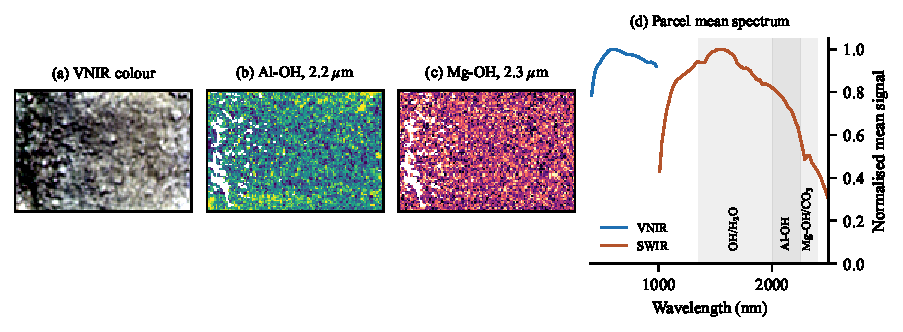
\includegraphics[width=0.86\textwidth]{figures/hsi_parcel_gmet0004.pdf}
\caption{One belt parcel as the hardness model sees it: HIDSAG composite GMET-0004 (Chilean porphyry Cu--Mo), 80$\times$117 pixels. (a) Colour image from the visible bands. (b, c) Relative absorption depth at the Al--OH (white mica, clays) and Mg--OH (chlorite, biotite, carbonate) features; detector stripes removed for display only. (d) Mean spectrum, with the absorption regions the model uses. The model predicts \Wi{} 15.9\,kWh/t with a 90\% upper bound of 16.9\,kWh/t (laboratory value 12.1\,kWh/t). The maps show absorption features, not a mineral identification.}
\label{fig:hsi}
\end{figure*}

Of the five HIDSAG targets tested (copper and molybdenum recovery, lime consumption, pH and Bond work index), only the work index beat its strongest baseline under every pass mark. Out of fold, the hyperspectral model explains 48\% of the variance in work index ($R^2$ 0.479, mean absolute error 1.05\,kWh/t), a model given only colour explains 21\% ($R^2$ 0.210, 1.29\,kWh/t), and the fold mean and median explain nothing ($R^2$ $-0.027$ and $-0.041$), so the infrared carries most of the information. Mean measured \Wi{} is 14.62\,kWh/t.



\begin{figure}[t]
\centering
\begin{tikzpicture}
\begin{axis}[
  scale only axis, width=5.6cm, height=3.2cm,
  xmin=11, xmax=22.5, ymin=11, ymax=22.5,
  xlabel={One-sided 90\% upper bound on \Wi{} (kWh/t)}, ylabel={Measured \Wi{} (kWh/t)},
  tick label style={font=\scriptsize}, label style={font=\footnotesize},
  axis lines*=left, grid=major, grid style={gray!15},
  legend style={at={(0.03,0.97)}, anchor=north west, font=\scriptsize, draw=none, fill=white},
  legend cell align=left]
\addplot[only marks, mark=*, mark size=1.1pt, accent, opacity=0.75] table[x=bound, y=measured] {figures/belt_bound_held.csv};
\addlegendentry{bound held (136)}
\addplot[only marks, mark=triangle*, mark size=2pt, red!75!black] table[x=bound, y=measured] {figures/belt_bound_exceeded.csv};
\addlegendentry{ore harder than bound (10)}
\addplot[black, dashed, domain=11:22.5, samples=2] {x};
\end{axis}
\end{tikzpicture}
\caption{Calibration of the hardness bound, out of fold, 146 composites (no drill-hole grouping available). Points below the dashed line are samples the bound covered: 93.2\% (95\% CI 88.4--96.6\%) against the 90\% target. The bound sits on average 1.64\,kWh/t (range 1.04--2.14) above the prediction.}
\label{fig:calibration}
\end{figure}

Figure~\ref{fig:calibration} illustrates how the bound behaves, highlighting that it was exceeded on 10 of 146 samples (6.8\%). The 95\% interval for coverage (88.4--96.6\%) spans the 90\% target, so the result is compatible with it but does not establish future coverage, particularly on new ore. The price of the bound is width: the bound sits on average 1.64\,kWh/t, about 11\% of the mean hardness, above the best guess. The OOD check passed 137 parcels, marked 5 borderline and refused 4. Figure~\ref{fig:hsi} shows one parcel as the model sees it. For parcel GMET-0004 the predicted \Wi{} is 15.9\,kWh/t and the bound 16.9\,kWh/t, against a design hardness of 16.6\,kWh/t (the training data's 90th percentile), so the proposal is 98.2\% of design feed. The laboratory value was 12.1\,kWh/t, so the bound was conservative here.

\subsection{Belt: from hardness to a plant decision}\label{sec:beltdecision}



Figure~\ref{fig:policies} illustrates four feed-rate policies replayed over all 146 composites against a fixed design-feed policy (the 90th-percentile hardness), highlighting the trade-off between throughput and overloads. In the replay a parcel is \emph{overloaded} when its true hardness exceeds the hardness the feed was set for; this is a model quantity, not a plant trip. Setting the feed from the bound, with OOD parcels withdrawn, gave a simulated throughput gain of +1.9\% (95\% CI +0.9 to +2.9\%), and the overload share was 6.8\% against 8.9\%; the one-sided 95\% upper bound on the difference (+1.4 points) is inside the +3-point margin in the evaluation plan. The original replay did not apply the 85--110\% envelope; a later analysis with it gives +1.7\% (+0.7 to +2.7\%) and the same overload share. Feeding from the best guess instead would add 13.6\% but overload 45.2\% of parcels, which is why the policy uses a bound. Perfect knowledge would add 14.0\%, so the bound captures about one-seventh of what is available: its width (1.64\,kWh/t) is where the rest is lost, and a tighter bound from site data is the main route to a larger gain.

\begin{figure}[t]
\centering
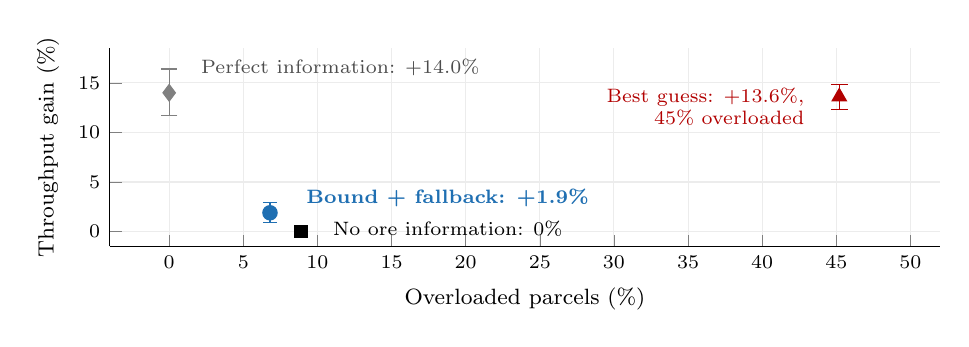
\begin{tikzpicture}
\begin{axis}[
  width=\columnwidth, height=4.1cm,
  xmin=-4, xmax=52, ymin=-1.5, ymax=18.5,
  xlabel={Overloaded parcels (\%)}, ylabel={Throughput gain (\%)},
  tick label style={font=\scriptsize}, label style={font=\footnotesize},
  axis lines*=left, grid=both, grid style={gray!15}]
\addplot[only marks, mark=square*, mark size=2.2pt, black, error bars/.cd, y dir=both, y explicit] coordinates {(8.9,0) +- (0,0)};
\addplot[only marks, mark=*, mark size=2.6pt, accent, error bars/.cd, y dir=both, y explicit] coordinates {(6.8,1.9) += (0,1.0) -= (0,1.0)};
\addplot[only marks, mark=triangle*, mark size=3pt, red!70!black, error bars/.cd, y dir=both, y explicit] coordinates {(45.2,13.6) += (0,1.2) -= (0,1.3)};
\addplot[only marks, mark=diamond*, mark size=3pt, gray, error bars/.cd, y dir=both, y explicit] coordinates {(0,14.0) += (0,2.4) -= (0,2.3)};
\node[font=\scriptsize, anchor=west] at (axis cs:10.4,0.25) {No ore information: 0\%};
\node[font=\scriptsize\bfseries, anchor=west, text=accent] at (axis cs:8.6,3.4) {Bound + fallback: +1.9\%};
\node[font=\scriptsize, anchor=east, align=right, text=red!70!black] at (axis cs:43.5,12.6) {Best guess: +13.6\%,\\45\% overloaded};
\node[font=\scriptsize, anchor=west, text=gray!60!black] at (axis cs:1.5,16.6) {Perfect information: +14.0\%};
\end{axis}
\end{tikzpicture}
\caption{Feed-rate policies replayed over 146 composites against a fixed design-feed policy (simulated; not PGM ore, not a time series, original replay without the envelope), with 95\% confidence intervals. Up is more throughput; left is fewer replay overloads.}
\label{fig:policies}
\end{figure}

The result is provisional for three reasons: the exact bound was adopted after the more efficient one failed, HIDSAG has no time order (so transit time, stockpile mixing and the asymmetric ramp limit are not simulated), and the ore is not Bushveld ore. Symmetric ramp limits were tested over 200 random parcel orders: $\pm$10\% per parcel left overloads unchanged ($-0.3$ points), but $\pm$5\% added 2.1 points and $\pm$2\% added 4.7, so feed must be cut fast. A predefined robustness test found the error unchanged for a new capture, half the field of view, added noise and $\pm$15\% illumination, but 1.25 times larger, unflagged, under wavelength drift, so a wavelength-calibration check was added.

\subsection{Is it physically possible?}\label{sec:physics}

Every claim was tested against its physics, and the failures stay in the report. In the evaluated flotation scenarios, grinding faster cost up to 0.25 percentage points of recovery on the steep part of the recovery curve and none on the plateau; this is the largest loss among the scenarios modelled, not a physical bound, and the site's recovery curve must be measured. Re-ordering ore during load-shedding cannot create tonnes, because energy per tonne is conserved over a cycle: it gave $-3.8\%$ in simulation, and even perfect knowledge gave $-3.0\%$, so that claim was rejected. The camera resolves parcels, not particles, and no test showed that it can identify minerals, so the microscope carries the phases.

\subsection{Laboratory: phase identification}\label{sec:micro}

\begin{figure}[t]
\centering
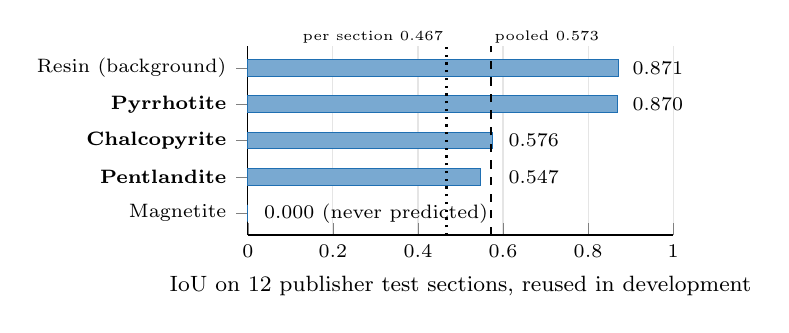
\begin{tikzpicture}
\begin{axis}[
  xbar, scale only axis, width=5.4cm, height=2.4cm, bar width=6pt, clip=false,
  xmin=0, xmax=1.0, ymin=0.4, ymax=5.6, ytick={1,...,5},
  yticklabels={Magnetite, \textbf{Pentlandite}, \textbf{Chalcopyrite}, \textbf{Pyrrhotite}, Resin (background)},
  y tick label style={font=\scriptsize}, x tick label style={font=\scriptsize, /pgf/number format/fixed},
  xlabel={IoU on 12 publisher test sections, reused in development}, label style={font=\footnotesize},
  axis lines*=left, xmajorgrids, grid style={gray!20}]
\addplot[fill=accent!60, draw=accent] coordinates {(0,1) (0.5468,2) (0.5755,3) (0.8695,4) (0.8709,5)};
\draw[black, dashed, thick] (axis cs:0.5725,0.4) -- (axis cs:0.5725,5.6);
\draw[black, dotted, thick] (axis cs:0.4671,0.4) -- (axis cs:0.4671,5.6);
\node[font=\scriptsize, anchor=west] at (axis cs:0.015,1) {0.000 (never predicted)};
\node[font=\scriptsize, anchor=west] at (axis cs:0.59,2) {0.547};
\node[font=\scriptsize, anchor=west] at (axis cs:0.59,3) {0.576};
\node[font=\scriptsize, anchor=west] at (axis cs:0.882,4) {0.870};
\node[font=\scriptsize, anchor=west] at (axis cs:0.882,5) {0.871};
\node[font=\tiny, anchor=south west, inner sep=1pt] at (axis cs:0.5725,5.6) {pooled 0.573};
\node[font=\tiny, anchor=south east, inner sep=1pt] at (axis cs:0.4671,5.6) {per section 0.467};
\end{axis}
\end{tikzpicture}
\caption{Microscope accuracy by class for the historically evaluated checkpoint \sha{de7135a9}, full-section inference on development-influenced sections; the pooled mean is over all five classes. The three phases the brief requires are in bold. Section means range from 0.340 to 0.728 (Appendix~\ref{app:micro}).}
\label{fig:iou}
\end{figure}

The microscope addresses the brief's three-phase requirement on analogue ore. Figure~\ref{fig:iou} illustrates its accuracy by class, highlighting IoU values of 0.87 for pyrrhotite, 0.58 for chalcopyrite and 0.55 for pentlandite (precision and recall in Appendix~\ref{app:micro}). The pooled mean IoU is 0.5725 (95\% CI 0.494--0.624); averaged per section it is 0.4671 (0.412--0.534). The model clearly beats trivial baselines (majority class 0.117; colour-only 0.395).

Magnetite, a fourth class the brief does not require, is never predicted. It is only 0.8\% of the test pixels: 78\% of it is labelled as resin, 17\% as pyrrhotite and 5\% as pentlandite. The last share is about 0.3\% of all pixels predicted as pentlandite, so magnetite barely moves the payload measures.

Three checkpoints exist and must not share scores (Table~\ref{tab:registry}). The figures above describe \sha{de7135a9}. The application build audited on 6 October ran \sha{fb78727d}, which the application itself marks as not approved. On one previously used section (test\_11, six fields), the audit compared that model's output with the expert masks: pixel accuracy was 64.1\%, pyrrhotite was predicted at 61.1\% of the area against 90.7\% in the reference, and pentlandite at 34.8\% against 2.0\%. This is one development section, not QEMSCAN and not an independent cohort, but it is a concrete counterexample to any blanket $\leq$10\% claim for the active model. A retrained candidate, \sha{42646cfa}, scores 0.632 overall and detects magnetite, but loses pyrrhotite and pentlandite and has pentlandite precision of only 0.50 (Appendix~\ref{app:micro}); it is quarantined, and the comparative decision safety of the checkpoints is untested.

\begin{table}[t]
\centering\footnotesize
\caption{Model registry. Scores are bound to one checkpoint each. As of 7 October 2026, no checkpoint has been frozen for an independent test.}
\label{tab:registry}
\begin{tabularx}{\columnwidth}{@{}L{1.35cm}YL{1.6cm}@{}}
\toprule
Checkpoint & Evidence & Status \\
\midrule
\sha{de7135a9} & Mean IoU 0.573 pooled, 12 development-influenced sections & Historical evaluated; research demo \\
\sha{fb78727d} & Mean IoU 0.454 (re-run); audit on test\_11: pixel accuracy 64.1\%, pentlandite 34.8\% vs 2.0\% & Active in audited build; not approved \\
\sha{42646cfa} & Mean IoU 0.632; pentlandite IoU 0.446, precision 0.50 & Candidate; quarantined \\
\bottomrule
\end{tabularx}
\end{table}

\subsection{Laboratory: decisions and grain evidence}\label{sec:grains}

Table~\ref{tab:decisions} compares the advice from the model's masks with the advice from the expert masks. The model produced 4 definite recommendations, 6 \emph{verify} outputs and 2 \emph{too few grains} outputs on the 12 sections, so its action coverage was 4 of 12 (33\%). No definite recommendation disagreed in the unsafe direction with the same advisor applied to expert masks. This is a small, development-influenced rule-agreement result: it does not validate the rules themselves, establish an independent unsafe-action rate or demonstrate plant safety. The one-sided 95\% upper bound of 22.1\% on 0 of 12 refers to all sections, not to risk when the system acts. Both the rules and the abstention thresholds need independent evaluation on the host stream. Only 4 definite actions occurred, so even an ideal independent 0 of 4 would bound the failure rate only at about 52.7\% (one-sided 95\%). The counts are for \sha{de7135a9}.

\begin{table}[t]
\centering\footnotesize
\caption{Decision-level confusion on the 12 publisher test sections (reused in development): advice from the expert mask (rows) against advice from the model's mask (columns). The advisor can also flag a reagent issue when the reject phase dominates; this happened once, on the expert mask only.}
\label{tab:decisions}
\begin{tabular}{@{}lccccc@{}}
\toprule
Expert mask $\backslash$ model & Grind & Continue & Verify & Too few & Total \\
\midrule
Grind finer & \cellcolor{okgreen!20}3 & 0 & 3 & 2 & 8 \\
Continue & 0 & \cellcolor{okgreen!20}1 & 2 & 0 & 3 \\
Adjust reagent & 0 & 0 & 1 & 0 & 1 \\
\midrule
Total & 3 & 1 & 6 & 2 & 12 \\
\bottomrule
\end{tabular}
\end{table}

It is important to note that the $\pm$0.335 verify band was calibrated on these same sections, so the agreement result is partly in-sample. On the 9 sections the payload rule governs, the result stays at 0 wrong for bands of $\pm$0.25 or wider, but one section becomes unsafe below that and two with no band, so the band must be re-set on independent pilot sections. A realistic exposure shift ($-35$ levels on each colour channel) changed the advice on 8 of 12 sections, so illumination control is also a pilot requirement.



The application's grain inspector lets a mineralogist audit the advice grain by grain; its ``free/locked'' labels overstate a 2D classifier, and relabelling them is planned, not implemented. In Quick mode 19 of 24 grains on test\_11 touch a field edge, so Quick-mode grain statistics are indicative until a border policy is set.

% =====================================================================
\section{Comparison with literature and limitations}

\subsection{Comparison with literature}

Published work supports the plausibility of the approach, not its validity here. Notole et al.\ \cite{notole2025} validated hyperspectral imaging and portable XRF against reference methods on Merensky Reef drill core scanned at the Council for Geoscience in Pretoria, with long-wave infrared as well as VNIR/SWIR sensing; that shows the sensing works on Bushveld material, not that our VNIR/SWIR hardness model does, and it is not a public paired conveyor dataset. The three sulphides the microscope classifies are the main base-metal sulphides of UG2 ore \cite{jones2005}, and our 50\% proxy line coincides with a boundary between middling classes in Mintek's liberation scheme \cite{moodley2026}, although that boundary does not by itself define free material. Mintek's AI optimisation raised a lead--zinc concentrator's throughput by 0.5\%, worth over US\$2 million (about R33\,million) a year \cite{mintek2025}, which shows that moves of this order are valued, not that this system would deliver them.

Four ideas were tested and withdrawn, and they mark where the method stops. The belt spectra did not predict QEMSCAN mineralogy once size fraction and process line were accounted for; a later grouped re-analysis of the same HIDSAG MINERAL1 data (99 records, 36 composites, already used in development) confirmed this: all records were within 10 absolute points, yet only 23--91\% of eligible records were within 10\% relative error depending on the phase, and a simple process-line baseline beat the spectral model for chalcopyrite and pyrite. The belt claim is therefore limited to hardness. Belt chemistry routed Bushveld PGE ore worse than the mine plan's seam label (balanced accuracy 0.79 against 0.82). The belt did not predict recovery, lime or pH better than a baseline. Plant tags never forecast concentrate silica an hour ahead better than the last laboratory assay.

\subsection{Limitations}

The following limitations apply, and (a), (b) and (e) block any investment decision until tested: (a) no South African ore has been evaluated, and a model trained on Chilean porphyry core may not transfer, because hardness also depends on silicification, grain size and fracturing; (b) the belt result is a replay of 146 composites without time order or drill-hole grouping, against a fixed design-feed policy rather than the plant's existing control, and a camera sees the belt surface, which may not represent the mass entering the mill; (c) the belt camera predicts hardness and does not identify minerals, and the microscope has not been trained on chromite or the silicates; (d) the 12 microscope sections guided development, and the historical checkpoint cannot be regenerated exactly; (e) the advisor's rules (including the pyrrhotite-reject and 50\% assumptions) are unvalidated for any host ore, its band was set on the evaluation sections, and payload-dominance is a 2D proxy, not liberation; (f) latency is measured on one laptop, the plant is a simulator, and economic benefit has not been attributed at any site; and (g) there is no fresh paired PGM validation, the active application checkpoint differs from the evaluated one, chromite and silicate classes are missing, and reference-laboratory uncertainty is not yet quantified. Compared with the abstract Mintek accepted, three things changed: the five Bushveld phases became three sulphides on an analogue ore, because no labelled Bushveld images existed; the QEMSCAN ``teacher'' became the pilot's reference-laboratory stream; and the fallback became the host's own operating procedure (the demonstration's 100\% design feed is not universally conservative, because it can raise feed from a lower running value).

% =====================================================================
\section{Business model and financial case}\label{sec:business}

\begin{figure*}[t]
\centering
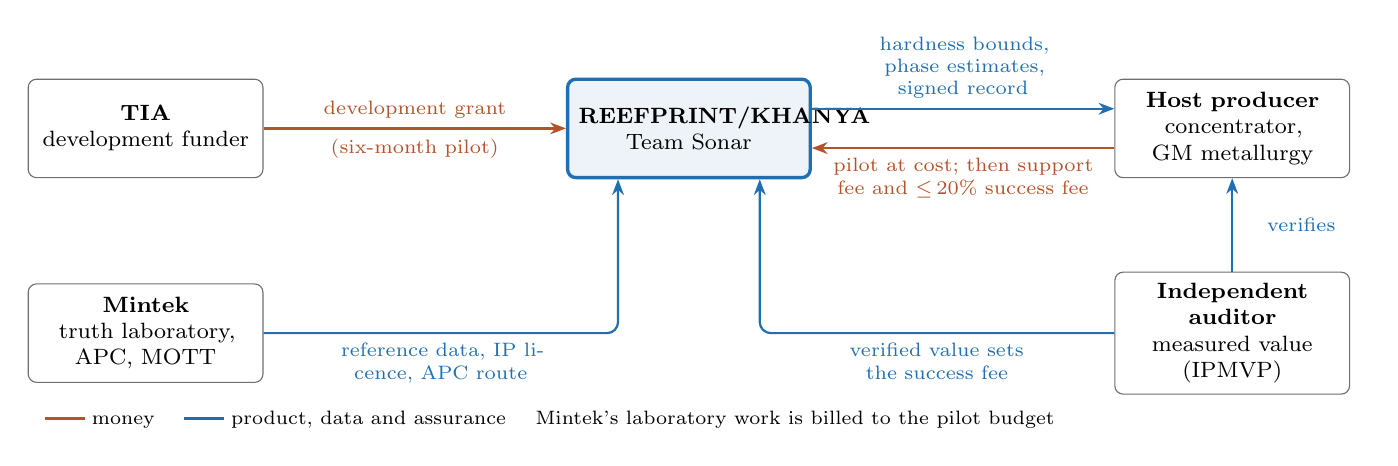
\begin{tikzpicture}[
  party/.style={draw=soft, rounded corners=3pt, align=center, text width=2.7cm, font=\footnotesize, inner sep=4pt, minimum height=1.25cm, fill=white},
  core/.style={draw=accent, very thick, rounded corners=3pt, align=center, text width=2.8cm, font=\footnotesize, inner sep=4pt, minimum height=1.25cm, fill=accent!8},
  money/.style={-{Stealth[length=2mm]}, thick, copper, rounded corners=4pt},
  value/.style={-{Stealth[length=2mm]}, thick, accent, rounded corners=4pt},
  lab/.style={font=\scriptsize, align=center, text width=3.4cm}]
\node[party] (tia) at (-6.9,0) {\textbf{TIA}\\ development funder};
\node[core] (team) at (0,0) {\textbf{REEFPRINT/KHANYA}\\ Team Sonar};
\node[party] (prod) at (6.9,0) {\textbf{Host producer}\\ concentrator, GM metallurgy};
\node[party] (mintek) at (-6.9,-2.6) {\textbf{Mintek}\\ truth laboratory, APC, MOTT};
\node[party] (mv) at (6.9,-2.6) {\textbf{Independent auditor}\\ measured value (IPMVP)};
\draw[money] (tia.east) -- node[lab, above] {development grant} node[lab, below] {(six-month pilot)} (team.west);
\draw[value] ([yshift=0.25cm]team.east) -- node[lab, above, text width=3.9cm] {hardness bounds, phase estimates,\\ signed record} ([yshift=0.25cm]prod.west);
\draw[money] ([yshift=-0.25cm]prod.west) -- node[lab, below, text width=3.9cm] {pilot at cost; then support fee and $\leq$\,20\% success fee} ([yshift=-0.25cm]team.east);
\draw[value] (mintek.east) -| node[lab, pos=0.25, below] {reference data, IP licence, APC route} ([xshift=-0.9cm]team.south);
\draw[value] (mv.west) -| node[lab, pos=0.25, below] {verified value sets the success fee} ([xshift=0.9cm]team.south);
\draw[value] (mv.north) -- node[lab, right, text width=1.5cm] {verifies} (prod.south);
\node[font=\scriptsize, anchor=west] at (-8.3,-3.7) {\textcolor{copper}{\rule[0.5ex]{0.5cm}{1.2pt}} money \quad \textcolor{accent}{\rule[0.5ex]{0.5cm}{1.2pt}} product, data and assurance \quad Mintek's laboratory work is billed to the pilot budget};
\end{tikzpicture}
\caption{The proposed business model; partner roles are proposals, not agreements. The pilot would be paid at cost; after a successful trial the producer would pay a fixed support fee and a success fee capped at 20\% of independently verified net value, which is zero when that value is zero or negative. Mintek would earn from the laboratory work the models need; licensing follows the hackathon IP agreement with its Office of Technology Transfer (MOTT).}
\label{fig:business}
\end{figure*}

\subsection{Value proposition and business model}

Our value proposition is simple: the plant gets a reading of its ore before the mill, with a stated bound, and beyond a fixed support fee it pays a success fee only on value that an independent party has measured. No producer, Mintek or TIA has agreed to fund, host or license the work; the roles below are proposals. The buyer is the concentrator manager or general manager for metallurgy at a South African PGM producer, who owns recovery, concentrate quality and mill throughput; producers such as Valterra, Implats, Sibanye-Stillwater, Northam and Tharisa are market segments, not customers. Figure~\ref{fig:business} illustrates how money and value flow, highlighting that the pilot is paid at cost and only the success fee depends on measured value. The Technology Innovation Agency (TIA), the national agency that funds technology development towards commercialisation \cite{tia}, is the proposed main funder of the pilot, subject to its criteria (Section~\ref{sec:tia}).

The proposed commercial structure has three parts: a fixed, capped validation contract for the research work; a separately agreed service fee after acceptance; and an optional variable fee capped at 20\% of independently verified net value, with the baseline, measurement period, adjustments, negative-value treatment and audit rights defined in advance. The success fee is zero when verified net value is zero or negative; validation charges and the support fee are separate, so no blanket zero-fee promise is made. Willingness to pay must still be tested through buyer interviews; laboratory savings are not claimed, because 4 definite decisions in 12 sections do not show that any paid analyses can be dropped. The model fits Mintek's published work \cite{mintek2025}: the models need QEMSCAN composites and Bond tests, which is laboratory work; Mintek's benefit-sharing model with Hindustan Zinc has generated over R35\,million since 2021; and its products reach over 60 countries through distributors. Valterra's realised basket price rose from R32,611 per ounce in 2025 to R45,993 in the first half of 2026 \cite{valterra2025,valterra2026}.

Plants already have cross-belt neutron analysers (bulk elements, with isotope sources that need a licence \cite{sahpra}), slurry analysers (grade after milling), automated mineralogy (phases, in days) and APC such as MillStar and FloatStar. The system replaces none of them; whether it adds ore-side information beyond APC, operator practice and mine-plan blending is what the pilot must show.

\subsection{What the money pays for}\label{sec:pricing}

Table~\ref{tab:pricing} sets out one scoped budget. The six-month pilot (Section~\ref{sec:pilotcost}) replaces the earlier R210,000 first tranche, and the earlier R8.2--49.2\,million installation grid survives only as a superseded sensitivity in Table~\ref{tab:sens}. Belt capital is a separate team allowance for one belt over about six months, released only after the belt-transfer gates (G1B and G1C); a pre-purchase scanner route is funded inside the pilot, so that G1B can be reached without buying the system it is meant to approve. VAT, duties, major civil work, conveyors or sorters, shutdown costs and closed-loop control are excluded and would be funded separately, so the totals are scoped budgets, not worst-case losses. After a trial, annual support is assumed at US\$30,000--60,000 (R0.49--0.98\,million), not added again to the six-month support line.

\begin{table*}[t]
\centering\footnotesize
\caption{One scoped budget: team planning allowances, not quotations. US\$ list prices are public anchors from one university facility and one industry guide, converted at R16.4 per US\$ (January--September 2026 average \cite{fred}); every line is replaced by a quote at G0.}
\label{tab:pricing}
\begin{tabularx}{\textwidth}{@{}L{4.15cm}L{1.25cm}Y|L{3.6cm}L{2.55cm}@{}}
\toprule
\multicolumn{3}{@{}l|}{\textbf{Six-month pilot (Section~\ref{sec:pilot})}} & \multicolumn{2}{l@{}}{\textbf{One belt, about six months (after G1B, G1C)}} \\
Item & Rand & Basis & Item & US\$ (rand) \\
\midrule
Two pilot engineers (the authors) & 480,000 & 2 $\times$ 6 months $\times$ R40,000 & Sensors, optics, references & 100--160k (R1.64--2.62\,M) \\
Software and OT-security engineer & 360,000 & To recruit; 6 months $\times$ R60,000 & Lighting, enclosure, mounting & 25--40k (R0.41--0.66\,M) \\
Independent mineralogist & 280,000 & 35 days $\times$ R8,000; annotates development specimens & Edge computer, UPS, network & 10--15k (R0.16--0.25\,M) \\
Statistician and data custodian & 144,000 & 18 days $\times$ R8,000 & Installation, integration, commissioning & 40--65k (R0.66--1.07\,M) \\
Site living, travel, medicals, inductions & 318,000 & 3 people $\times$ 6 months; PPE & Sampling, reference, support & 25--40k (R0.41--0.66\,M) \\
Polished-section preparation & 154,000 & 77 sections $\times$ R2,000 & 25\% contingency & 50--80k (R0.82--1.31\,M) \\
Automated mineralogy & 1,443,000 & 44 specimens $\times$ US\$2,000 list \cite{camp} & \textbf{Total} & \textbf{250--400k (R4.10--6.56\,M)} \\
Bond ball-mill work index & 866,000 & 44 composites $\times$ up to US\$1,200 \cite{bondcost} & & \\
Scanner access (rental or vendor laboratory) & 300,000 & Allowance; no quote yet & & \\
Microscope imaging kit, edge computer, UPS & 120,000 & Allowance & & \\
Independent review, IP and data terms, close-out & 120,000 & Allowance & & \\
Contingency (15\%) & 688,000 & Released only on a documented risk event & & \\
\textbf{Total pilot} & \textbf{5,273,000} & No overrun without a new decision & \textbf{Pilot plus belt stage} & \textbf{R9.37--11.83\,M} \\
\bottomrule
\end{tabularx}
\end{table*}

\subsection{From throughput to recovered metal}\label{sec:value}

The belt result is a throughput gain, and revenue comes from recovered metal, so the two must be bridged. For a consistent stream, metal output is proportional to dry tonnes $\times$ head grade $\times$ recovery, so
\begin{equation}
\frac{\Delta M}{M} = \Big(1+\frac{\Delta T}{T}\Big)\Big(1+\frac{\Delta G}{G}\Big)\Big(1+\frac{\Delta R}{R}\Big) - 1 ,
\end{equation}
where $T$ is throughput, $G$ head grade and $R$ recovery. With unchanged grade, a 1.75\% throughput gain and a recovery loss of 0.25 percentage points from 87\% (a relative change of $-0.29\%$) give 1.46\% more metal. Where the plant is limited by ore supply, extra throughput is worth nothing. If all of Zondereinde's output passed the instrumented circuit (an upper bound), 1.46\% more metal would be worth R64--123\,million a year in margin, and a quarter of that gain R16--31\,million; these are simulated gains, not measurements.



\subsection{Financial methodology}\label{sec:finance}

The following assumptions apply: (a) annual output is that of Northam's Zondereinde mine, 333,050 equivalent refined 4E ounces in F2026 \cite{northam2026}; (b) prices are Valterra's realised basket prices of R32,611 per ounce (2025) and R45,993 (first half of 2026), with cash operating costs of R19,488 and R20,677 per ounce \cite{valterra2025,valterra2026}, used as proxies for another company's mine, with different baskets, payability and cost structure; (c) for a commercial-life case, installed cost is the belt allowance without the six-month support line (US\$175,000--280,000, R2.87--4.59\,million) and running cost is the post-trial support (R0.49--0.98\,million a year); (d) the equipment has a 5-year life at a 10\% discount rate; and (e) an affected-output fraction $f$ of the mine's output passes the instrumented circuit, taken as 1 unless stated. The annual value of an uplift $u$ in recovered metal is
\begin{equation}
V = u \times f \times Q \times m ,
\end{equation}
where $Q$ is annual output in ounces and $m$ the margin per ounce. For $u$ = 1\% and $m$ = price less cash cost,
\begin{equation}
V = 0.01 \times 333{,}050 \times (\text{R}13{,}123 \text{ to } \text{R}25{,}316),
\end{equation}
which is equivalent to R43.7--84.3\,million a year (R108.6--153.2\,million in revenue before costs). Deducting the full average cash cost may be conservative where the mill has spare capacity, but extra mining, handling or bottleneck costs could change that, so a host-approved incremental cash-flow model is needed before investment. The installed cost is spread over the equipment's life with the capital recovery factor
\begin{equation}
\text{CRF} = \frac{r(1+r)^n}{(1+r)^n-1} = 0.2638 \quad (r = 10\%,\ n = 5),
\end{equation}
so the annualised cost is
\begin{equation}
C = \text{CRF} \times C_{\text{installed}} + C_{\text{running}},
\end{equation}
which is equivalent to R1.25--2.20\,million a year, or R2.50\,million with the 25\% contingency on the high case. The break-even uplift is then $u_{\text{BE}} = C/(f \times Q \times m)$. Table~\ref{tab:sens} shows how it moves with cost, margin, affected fraction and the fee basis. If the 20\% fee is charged on the margin before system costs, the producer breaks even only when $0.8\,V = C$. The break-even figures are far smaller than the precision with which a short plant trial can measure uplift, which is why measured value, not break-even, decides G5.

\begin{table}[t]
\centering\footnotesize
\caption{Break-even sensitivities in relative recovered metal (recalculated under the stated assumptions; illustrative, not a site funding threshold). One percentage point of recovery at 80\% recovery is 1.25\% relative.}
\label{tab:sens}
\begin{tabularx}{\columnwidth}{@{}YL{1.35cm}@{}}
\toprule
Scenario & More metal needed \\
\midrule
Low cost, 2026 margin, all output affected & 0.015\% \\
High cost, 2025 margin, all output & 0.050\% \\
High cost + 25\% contingency, 2025 margin & 0.057\% \\
High cost, 2025 margin, 20\% fee before system costs & 0.063\% \\
High cost, 2025 margin, half of output affected & 0.10\% \\
High cost, 2025 margin, a quarter of output affected & 0.20\% \\
High cost, 30\% lower basket price (2025 costs) & 0.20\% \\
\midrule
Superseded R49.2\,M installation grid, 2025 margin & 0.52\% \\
\bottomrule
\end{tabularx}
\end{table}


Annualising over five years describes continued successful use, not whether a six-month pilot pays for itself. The pilot cash view is simpler: the pilot is a research cost of at most R5.27\,million, released in tranches so that a stop at any review leaves later tranches unspent; no belt equipment is ordered before G1B and G1C; and if the belt stage proceeds and then stops, the exposure is up to R9.37--11.83\,million, with equipment resale assumed to be zero in the pessimistic case. The fee basis must be agreed so that no support cost is charged twice, and measured value needs an agreed metallurgical accounting boundary and attribution method under IPMVP \cite{ipmvp}.

% =====================================================================
\section{The six-month pilot}\label{sec:pilot}

As Team Sonar, our pilot problem is this: in six months at one host concentrator, find out whether the microscope meets a $\leq$10\% phase-abundance target on independent local specimens, and whether the hardness model transfers to local ore, before anyone buys belt equipment. Everything after the pilot depends on its evidence, and a clear negative answer is a useful result.

\subsection{Why six months is feasible}

The following assumptions make six months realistic: (a) contracting (host letter, stream, quotes, scanner access, data and IP terms, signed acceptance contract) is finished before month~0 at gate G0, so the clock starts at a readiness event, not a funding announcement; (b) no belt hardware is bought or installed: the microscope runs on a laptop, and belt spectra are taken from host samples on a rented or vendor-laboratory scanner; (c) specimens come from the host's existing shift sampling, so 70 microscope specimens and 44 Bond composites over 14 collection weeks need only about 5 and 3 a week; (d) reference results return in fortnightly batches within an agreed three weeks, so the last batch is back before the locked evaluation in month~5; and (e) the software, model registry and abundance-error checks already exist, so the time goes on evidence, not on building. If sample supply or laboratory turnaround slips, the pilot is extended; the cohort is never cut to keep the date.

\subsection{What the pilot must achieve}\label{sec:goals}

Table~\ref{tab:goals} sets out the proposed targets, to be signed with the host before any evaluation specimen is collected. We use ``90\% accuracy'' in one strict sense: at least 90\% of locked specimens must meet the error contract for every decision-critical phase. With 30 locked specimens, an observed 27 of 30 shows only that the true pass rate exceeds 76\% (one-sided 95\%); demonstrating 90\% itself needs 29 of 29, or 45 of 46 if one failure is allowed. We fund 30 and report the lower bound; enlarging the locked set to 46 would add about R0.56\,million before contingency.

\begin{table}[t]
\centering\footnotesize
\caption{Proposed pilot targets. ``Agreed'' values are signed with the host and statistician before evaluation specimens are collected.}
\label{tab:goals}
\begin{tabularx}{\columnwidth}{@{}L{1.45cm}YL{0.75cm}@{}}
\toprule
Target & Pass condition (proposed) & Gate \\
\midrule
Phase abundance & Pentlandite, chalcopyrite, pyrrhotite: $\leq$10\% relative error above an agreed reporting limit, absolute tolerance below it; $\geq$27 of 30 locked specimens pass, lower bound reported & G1A \\
Coverage & Refusals and failures stay in the denominator; answered share $\geq$ agreed minimum & G1A \\
Hardness transfer & 44 host composites: out-of-fold error below a metadata baseline; 90\% bound coverage with its interval spanning 90\%; agreed width & G1B \\
Moving bed & Error on moving, moist, unsorted ore within an agreed ratio of the static result & G1C \\
Shift routine & 3-week shadow run in the host laboratory: turnaround, refusals, record integrity; nobody acts & TRL~6 \\
\bottomrule
\end{tabularx}
\end{table}

\subsection{Work plan and a day on site}

\begin{figure*}[t]
\centering
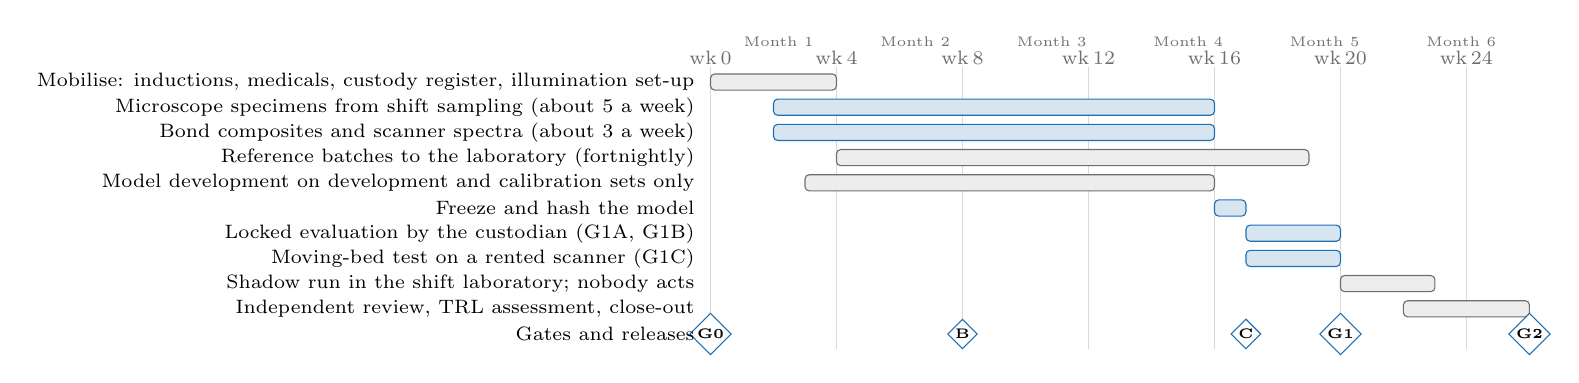
\begin{tikzpicture}[x=0.4cm, y=0.32cm,
  bar/.style={draw=soft, fill=gray!14, rounded corners=1.5pt},
  hot/.style={draw=accent, fill=accent!18, rounded corners=1.5pt},
  gate/.style={draw=accent, fill=white, diamond, aspect=1, inner sep=0.5pt, minimum size=0.36cm, font=\tiny\bfseries}]
\foreach \w in {0,4,8,12,16,20,24} { \draw[gray!30] (\w,0.6) -- (\w,-10.6); \node[font=\scriptsize, soft] at (\w,0.95) {wk\,\w}; }
\foreach \m in {1,...,6} { \node[font=\tiny, soft] at ({(\m-0.5)*26/6},1.6) {Month \m}; }
\foreach \r/\t in {0/{Mobilise: inductions, medicals, custody register, illumination set-up}, 1/{Microscope specimens from shift sampling (about 5 a week)}, 2/{Bond composites and scanner spectra (about 3 a week)}, 3/{Reference batches to the laboratory (fortnightly)}, 4/{Model development on development and calibration sets only}, 5/{Freeze and hash the model}, 6/{Locked evaluation by the custodian (G1A, G1B)}, 7/{Moving-bed test on a rented scanner (G1C)}, 8/{Shadow run in the shift laboratory; nobody acts}, 9/{Independent review, TRL assessment, close-out}}
  { \node[font=\scriptsize, anchor=east] at (-0.2,-\r) {\t}; }
\foreach \r/\a/\b/\s in {0/0/4/bar, 1/2/16/hot, 2/2/16/hot, 3/4/19/bar, 4/3/16/bar, 5/16/17/hot, 6/17/20/hot, 7/17/20/hot, 8/20/23/bar, 9/22/26/bar}
  { \draw[\s] (\a,-\r-0.32) rectangle (\b,-\r+0.32); }
\foreach \x/\g in {0/G0, 8/B, 17/C, 20/G1, 26/G2} { \node[gate] at (\x,-10.0) {\g}; }
\node[font=\scriptsize, anchor=east] at (-0.2,-10.0) {Gates and releases};
\end{tikzpicture}
\caption{The six-month pilot, in weeks from the readiness event (planning estimate). Shaded blue bars are evidence-producing work. Diamonds: G0 releases tranche A; B is the week-8 review that releases tranche B; C releases tranche C once the model is frozen; G1 marks the G1A, G1B and G1C decisions; G2 is the decision on the belt stage. No belt equipment is ordered inside the pilot.}
\label{fig:pilotplan}
\end{figure*}

Figure~\ref{fig:pilotplan} illustrates the plan, highlighting that the model is frozen before any locked reference is revealed. A typical day on site would run as follows (proposed; the host sets the hours and safety rules):
\begin{enumerate}[label=(\roman*)]
\item shift handover and safety talk; collect the previous shift's sampler cuts with the host's sampling crew and log each in the custody register;
\item split each cut into a section split, a Bond-composite split and a retained split; scan the Bond splits; the custodian's script, not the team, assigns each specimen to development, calibration or locked;
\item image the returned polished sections under controlled light with a colour reference; the frozen model's outputs on locked images are hashed and sealed before any reference is seen;
\item development work only on development and calibration specimens; data-quality, fault and refusal logs;
\item a short review with the host metallurgist; back up and sign the day's records.
\end{enumerate}
Each week a reference batch is dispatched and the mineralogist reviews annotations; each month a steering meeting checks spend, risks and schedule against the gates.

\subsection{The team to assemble}

Table~\ref{tab:team} lists the people the pilot needs. The two authors are in place; the software and operational-technology (OT) security engineer must be recruited before G0, and the independent roles are contracted, so that assessment never collapses into self-certification. The host owns plant operation and stop authority, and nothing in the pilot writes to the plant.

\begin{table}[t]
\centering\footnotesize
\caption{The pilot team (functions; one person may cover several, except the independent ones).}
\label{tab:team}
\begin{tabularx}{\columnwidth}{@{}L{2.15cm}L{1.35cm}Y@{}}
\toprule
Role & Time & During the pilot \\
\midrule
Pilot lead, field and systems (S.~Khumalo) & Full time, on site & Sampling, custody, imaging, integration, reporting \\
Model and evaluation lead (L.~Hoaeane) & Full time & Model development and freeze, abundance contract, belt-transfer analysis \\
Software and OT-security engineer & To recruit; full time & Release manifest, offline operation, security, signed record \\
Independent mineralogist & About 35 days & Annotates development specimens, reviews references, phase taxonomy \\
Statistician and data custodian & About 18 days & Blind split, sealed predictions, power check, evaluation \\
Host metallurgist; safety and OT officers & Host, in kind & Use case, sampling access, inductions, risk assessment, sign-off \\
Reference laboratory & Quoted & Section preparation, automated mineralogy, Bond tests \\
\bottomrule
\end{tabularx}
\end{table}

\subsection{What the pilot costs, and why R210,000 was too low}\label{sec:pilotcost}

The earlier first tranche of R210,000 paid for laboratory work, not for a pilot. Its R65,000 reference line over 70 specimens allowed about R929 a specimen, whereas one published university list price for automated mineralogy is US\$1,500--2,000 a sample (R24,600--32,800) \cite{camp} and a Bond ball-mill test typically costs up to about US\$1,200 (R19,700) \cite{bondcost}. It also paid nobody to be on site, no accommodation, inductions or medicals, and no scanner access for the belt-transfer test, so its loss cap depended on unfunded work. The left half of Table~\ref{tab:pricing} replaces it with a bottom-up budget of R5.27\,million. To keep it lean, the 30 development specimens are referenced by expert annotation, and only the 10 calibration, 30 locked and 4 duplicate specimens go to automated mineralogy. Staff rates are team planning rates, and every line is replaced by a quote at G0; if quotes exceed the ceiling, the question is narrowed or returned for a new decision, never quietly cut.

Money is released in three tranches: A, R1.00\,million at G0 (two months of staff, imaging kit, inductions, scanner booking); B, R3.08\,million at the week-8 review, once sampling and custody work and quotes are accepted (reference programme and scanner time); and C, R0.50\,million after the model is frozen (evaluation and close-out). The R0.69\,million contingency is released only against a documented risk event. Laboratory orders already placed are the main cost that a stop decision cannot recover.

\subsection{How TIA fits}\label{sec:tia}

TIA funds technology from proof of concept (TRL~3) to pre-commercialisation (TRL~8), with instruments matched to readiness \cite{tiafund}. Its Technology Development Fund covers TRL~4--7 and lists demonstration and pilot plants and techno-economic studies as fundable, so it fits this pilot. The Seed Fund covers TRL~5--6, up to R1.5\,million over 12--24 months, and excludes TRL~3--4 projects \cite{tiaseed}, so it fits a later productisation of the microscope, not the pilot. Seed applicants need a functional prototype with a technical report, a technology roadmap, an industry partner and an IP strategy \cite{tiaseed}; we have the first two, and the other two are G0 items. Beyond money, TIA links innovators with technology-transfer offices, incubators and investors \cite{tiafund}. Table~\ref{tab:tia} sets out the proposed structure; no application has been made and no amount is agreed.

\begin{table}[t]
\centering\footnotesize
\caption{Proposed funding structure around TIA (proposals; nothing is agreed).}
\label{tab:tia}
\begin{tabularx}{\columnwidth}{@{}L{1.3cm}L{0.75cm}L{1.95cm}Y@{}}
\toprule
Stage & TRL & TIA instrument & Cash and other parties \\
\midrule
Six-month pilot & 3--4 to 4--6 & Technology Development Fund & TIA R4.28\,M; host pays Bond tests (R1.00\,M with contingency) and gives site access, metallurgist time and laboratory space; Mintek reference work at cost \\
Microscope product & 5--6 & Seed Fund, via a university office & Up to R1.5\,M; technology-transfer office and incubator \\
One belt & 6--7 & Development Fund or Industry Matching Fund & R4.10--6.56\,M, co-funded by the host \\
Roll-out & 8--9 & Commercialisation Support & Not set; investors \\
\bottomrule
\end{tabularx}
\end{table}

\subsection{Pilot risks and mitigations}\label{sec:risks}

Table~\ref{tab:risks} sets out the risks of the pilot period, as the team assesses them, each with a mitigation before it happens and a fallback if it does. Contingency pays only for uncertain costs inside the approved scope. Risks of later use (belt dust and drift, cyber attack, operator over-reliance, no measured gain, price falls) are handled by gates G2--G5, read-only advisory tags, IEC~62443 zones \cite{iec62443} and a success fee that falls with value.

\begin{table*}[t]
\centering\footnotesize
\caption{Pilot-period risk register: mitigation before the event, and the fallback if it happens.}
\label{tab:risks}
\begin{tabularx}{\textwidth}{@{}L{0.45cm}L{4.6cm}YY@{}}
\toprule
\# & Risk during the pilot & Mitigation (before) & Fallback (if it happens) \\
\midrule
P1 & Fewer than 5 specimens a week (stoppages, sampler faults) & Sampling plan agreed at G0; collect across shifts; weekly count & Extend collection; never shrink the locked cohort \\
P2 & Laboratory turnaround over 3 weeks, or quotes above budget & Turnaround written into the quote; fortnightly batches; second laboratory pre-qualified & Narrow the question or seek a new decision; no silent cuts to repeats \\
P3 & No scanner rental or vendor-laboratory time & Booking and quote at G0; two vendors approached & Belt track paused; microscope track continues \\
P4 & The model misses the $\leq$10\% target on locked specimens & Development and calibration sets used fully; one frozen model & Report the negative result; stop or narrow; locked set becomes development material \\
P5 & Leakage between development and locked sets & Independent custodian; split-integrity checks; sealed predictions & Withdraw the affected claim; collect a fresh cohort \\
P6 & Illumination or preparation drift & Colour reference on every image; preparation duplicates & Refuse affected images; re-image \\
P7 & Engineer not recruited, or a team member unavailable & Recruit before G0; named deputies; written runbooks & Hold tranche B; seek in-kind university support \\
P8 & Site access delays (medicals, inductions, stand-downs) & Medicals and inductions budgeted in month 1; host escort & Shift work to the laboratory; extend \\
P9 & Load-shedding or network loss & Offline laptop with UPS; local backups & Resume after checks; log the gap \\
P10 & Host withdraws, or data and IP terms unsigned; LumenStone rights unclear & Signed letter and IP and data schedule at G0; ask the rights holder & No further release; keep lawful evidence; qualify another host \\
P11 & Rand 10\% weaker on US\$-priced lines & Rand quotes where possible & Adds about R0.26\,M; covered by contingency \\
P12 & Safety incident on site & Host induction and PPE; no work near moving plant without an escort & Stop work; follow the host's procedure \\
\bottomrule
\end{tabularx}
\end{table*}

\subsection{Governance, compliance and training}

These are planned controls, not achieved compliance (Table~\ref{tab:compliance}). The Mine Health and Safety Act requires a risk assessment with the health and safety committee, and training before significant changes to plant \cite{mhsa}; POPIA governs approvers' names in the record \cite{popia}; Mining Charter clause 2.3.1 counts skills and R\&D spend \cite{charter2018}; IP from public funding falls under the IPR Act \cite{ipract}, although the contract, not the Act's name, settles ownership; and Mintek and TIA spend under the PFMA \cite{pfma}. Independent checks are outsourced: (a) a laboratory accredited by SANAS for the specific method \cite{sanas}; (b) Mintek's QEMSCAN for mineralogy; (c) an independent auditor for value, with a measurement plan adapted from IPMVP \cite{ipmvp}; (d) an IEC~62443 assessor; (e) an IP attorney through MOTT; and (f) a university reviewer for the model audit. Each group is trained before its phase, aligned with the site's skills plan \cite{mqa}: laboratory staff (one day, before G1A), metallurgists (one day, at G0), and later operators, technicians and IT/OT staff before G2--G4; competence is shown by observed tasks and sign-off, not attendance.

% =====================================================================
\section{TRL milestones and gates}\label{sec:roadmap}

Table~\ref{tab:trl} places each component on the standard readiness scale \cite{trl} and shows how each step is earned. A level is awarded only from evidence, by the independent reviewer, not from elapsed time. The microscope can climb faster because it needs no plant hardware; the belt model must cross three transfer steps: host samples on a laboratory scanner (G1B), a moving bed (G1C), and a host belt in shadow (G3).

\begin{table}[t]
\centering\footnotesize
\caption{TRL now, and the evidence that would earn each next level.}
\label{tab:trl}
\begin{tabularx}{\columnwidth}{@{}L{1.35cm}L{1.75cm}YL{1.1cm}@{}}
\toprule
Component & Now & End of pilot, if gates pass & Belt stage \\
\midrule
Microscope workflow & 4: validated in the laboratory on public analogue data & 5: independent host specimens (G1A); 6: shift shadow run & 6--7 \\
Belt hardness model & 3: proof of concept on public core; simulated plant & 4: host samples, laboratory scanner (G1B); 5: moving bed (G1C) & 6 (G3), 7 (G5) \\
Decision layer and record & 4: built; replayed data; simulated plant & 4 (not tested in the pilot) & 6--7 \\
\bottomrule
\end{tabularx}
\end{table}

Table~\ref{tab:milestones} lists what each gate must show, who decides, and what happens if it fails. After the pilot, a one-belt stage of about six months (G2--G5) follows only if G1B and G1C pass, so a commercial decision is about 12--18 months from the readiness event. A first pilot that ends with ``we found a narrower valid use and stopped an unjustified purchase'' should count as successful de-risking.

\begin{table}[t]
\centering\footnotesize
\caption{Gates, decision owners and stop outcomes. Numerical thresholds are signed before evaluation data are collected.}
\label{tab:milestones}
\begin{tabularx}{\columnwidth}{@{}L{0.55cm}YL{1.45cm}L{1.35cm}@{}}
\toprule
Gate & Release condition & Decides & If it fails \\
\midrule
G0 & Host letter, stream, quotes, scanner access, data and IP terms, signed contract & Funder, host sponsor & Fund preparation only \\
G1A & Microscope targets met on locked specimens (Table~\ref{tab:goals}) & Independent reviewer, host metallurgist & Research image review only \\
G1B & Hardness transfers to host samples & Same & Stop belt track \\
G1C & Transfer holds on a moving bed & Same & Reversible instrument trial only \\
G2 & Sensor quote, factory and site acceptance, risk assessment, read-only design & Host OT and safety leads & Repair or remove \\
G3 & Timing, paired sampling, drift, refusals in shadow; site recovery curve measured & Host metallurgist & Extend or stop \\
G4 & Envelope, change management, training, rollback & Host change board & Revert to host procedure \\
G5 & Independently measured net value and total cost & Auditor, host & Close out; no success fee \\
\bottomrule
\end{tabularx}
\end{table}


\begin{table*}[t]
{\fontsize{7}{8.3}\selectfont\renewcommand{\arraystretch}{0.92}\setlength{\extrarowheight}{0pt}\captionsetup{font=footnotesize,skip=2pt}
\begin{minipage}[t]{0.50\textwidth}
\captionof{table}{Microscope per-class results, historical checkpoint against the retrained candidate, 12 S2 publisher test sections reused in development (full-section inference).}
\label{tab:perclass}
\centering
\begin{tabular}{@{}lcccc@{}}
\toprule
& \multicolumn{3}{c}{Historical \sha{de7135a9}} & Candidate \\
Class & IoU & Recall & Precision & IoU (precision) \\
\midrule
Resin & 0.871 & 0.920 & 0.942 & 0.848 (0.960) \\
Chalcopyrite & 0.576 & 0.716 & 0.746 & 0.800 (0.937) \\
Magnetite & 0.000 & 0.000 & -- & 0.248 (0.255) \\
Pyrrhotite & 0.870 & 0.934 & 0.926 & 0.818 (0.950) \\
Pentlandite & 0.547 & 0.742 & 0.675 & 0.446 (0.503) \\
\midrule
Mean & 0.573 & & & 0.632 \\
\bottomrule
\end{tabular}
\end{minipage}\hfill
\begin{minipage}[t]{0.46\textwidth}
\captionof{table}{Pixel confusion for the historical checkpoint (\% of each true class), 103.8 million pixels.}
\label{tab:confusion}
\centering
\begin{tabular}{@{}lccccc@{}}
\toprule
True $\backslash$ predicted & Resin & Ccp & Mag & Po & Pn \\
\midrule
Resin & \cellcolor{accent!35}92.0 & 0.8 & 0.0 & 5.7 & 1.5 \\
Chalcopyrite & 1.6 & \cellcolor{accent!30}71.6 & 0.0 & 3.1 & 23.7 \\
Magnetite & 78.3 & 0.1 & 0.0 & 16.8 & 4.8 \\
Pyrrhotite & 1.1 & 1.6 & 0.0 & \cellcolor{accent!35}93.4 & 3.9 \\
Pentlandite & 0.7 & 0.8 & 0.0 & 24.3 & \cellcolor{accent!30}74.2 \\
\bottomrule
\end{tabular}
\end{minipage}\par}
\par\vspace{4pt}
{\fontsize{7}{8.3}\selectfont\renewcommand{\arraystretch}{0.92}\setlength{\extrarowheight}{0pt}\captionsetup{font=footnotesize,skip=2pt}
\begin{minipage}[t]{0.555\textwidth}
\captionof{table}{Laws, policies and standards, and the planned controls (not achieved compliance).}
\label{tab:compliance}
\begin{tabularx}{\linewidth}{@{}L{3.3cm}Y@{}}
\toprule
Law, policy or standard & What it asks, and the planned control \\
\midrule
Mine Health and Safety Act 29 of 1996 \cite{mhsa} & Risk assessment with the health and safety committee (s.~11, s.~34), training before significant plant changes (s.~10): site risk assessment and lockout; advisory only; trained operators \\
Protection of Personal Information Act 4 of 2013 \cite{popia} & Limited processing of approvers' names: purpose, access, retention and non-disciplinary use agreed with the information officer \\
Mining Charter 2018, clause 2.3.1 \cite{charter2018} & 5\% of the leviable amount on skills, including R\&D: pilot training and R\&D may count \\
IPR from Publicly Financed R\&D Act 51 of 2008 \cite{ipract} & IP identified and protected for South Africa: managed by MOTT under the hackathon agreement \cite{faq}, subject to the contract \\
Public Finance Management Act 1 of 1999 \cite{pfma} & Mintek (Schedule 3B) and TIA (3A) spend under PFMA controls: tranches tied to gates, auditable deliverables \\
Hazardous Substances Act 15 of 1973 \cite{sahpra} & Licences for radioactive sources: not applicable, optical sensing only \\
IEC 62443 \cite{iec62443}; OPC UA \cite{opcua} & Industrial cyber security zones: read-only advisory tags; no write path to safety systems \\
ISO/IEC 17025, SANAS \cite{sanas} & Laboratory competence: reference tests from laboratories accredited for that method \\
IPMVP (EVO) \cite{ipmvp} & Measurement and verification: success fee only on value verified under an agreed plan \\
\bottomrule
\end{tabularx}
\end{minipage}\hfill
\begin{minipage}[t]{0.425\textwidth}
\captionof{table}{Glossary.}\label{app:glossary}
\begin{tabularx}{\linewidth}{@{}L{1.9cm}Y@{}}
\toprule
APC & Advanced process control, e.g.\ Mintek's MillStar and FloatStar \\
Bond work index (\Wi{}) & Energy needed to grind ore, in kWh/t; harder ore has a higher \Wi{} \\
Bound & Here, a hardness the true value should stay below 9 times in 10 (one-sided 90\% conformal bound) \\
Fallback & In the demonstration, 100\% of design feed; at a site, the host's own operating policy under its existing controls \\
Deadband & The smallest change worth showing the operator \\
Envelope & The range of feed rates the site's metallurgist allows (demonstration: 85--110\% of design) \\
Payload-dominant & A grain at least half payload by 2D area (``free'' in the app); a proxy, not liberation \\
TRL & Technology readiness level, 1 (basic principles) to 9 (proven in operation) \cite{trl} \\
IoU & Intersection over union: overlap of predicted and expert areas, 0 to 1 \\
Parcel & 30\,s of belt in the pilot design; one composite scan in the replay \\
PGM, 4E & Platinum-group metals; 4E = Pt, Pd, Rh and Au \\
QEMSCAN & Automated scanning-electron mineralogy \\
SWIR, VNIR & Short-wave and visible--near infrared light \\
\bottomrule
\end{tabularx}
\end{minipage}\par}
\end{table*}

% =====================================================================
\section{Conclusions and recommendation}

The present contribution is a functioning, inspectable evidence workflow and a falsifiable route to local validation. On public analogue data the hardness model improves on simple baselines and the microscope classifies three relevant sulphide phases, but the feed-rate benefit is a simulation, the microscope results are development-influenced, the active application checkpoint has shown large abundance errors on one section, and the $\leq$10\% error target is untested. We therefore recommend a six-month pilot at one host concentrator, costed at R5.27\,million and funded mainly through TIA's Technology Development Fund in three tranches, with the $\leq$10\% error target tested on at least 30 locked host specimens and belt capital only after separate transfer gates. A clear negative result from the pilot is a useful outcome: it stops an unjustified purchase. As of this submission, the independent local phase-abundance target has not been demonstrated; a commercial claim will depend on independent reference agreement, useful acceptance coverage and measured net value on the affected stream.

% =====================================================================
\small
\backsec{CRediT authorship contribution statement.}
\textbf{Lethabo Hoaeane:} Conceptualisation, domain lead, belt hyperspectral modelling, belt monitor and decision application, economics, presentation. \textbf{Sibusiso Khumalo:} Microscope segmentation model, accuracy and decision-level evaluation, advisor and safety gates, OPC~UA simulation, workbench review and verification, technical report.

\backsec{Declaration of competing interest.}
The authors declare no known competing financial interests or personal relationships that could have appeared to influence the work reported in this paper.

\backsec{Acknowledgements.}
We thank the Mintek mentors for a review session that reshaped the build.

\backsec{Use of AI tools.}
Code and drafting were assisted by AI coding assistants. Every reported number was computed by code in the project repository and checked by the authors.

\backsec{Data and code availability.}
{\raggedright HIDSAG is available under CC0 (doi:10.6084/m9.figshare.c.5983921) \cite{ehrenfeld2023}; LumenStone under research-use terms \cite{korshunov2025}; the Bushveld assays under CC BY 4.0 (doi:10.17632/dc8jcnbcvk.1) \cite{bachmann2019}. Code, checkpoint hashes and every results file behind the numbers in this report: \url{https://github.com/Sibusiso-K/KHANYA} (Appendix~\ref{app:repro}). A static demonstration of the belt monitor runs at \url{https://lethabomh14-reefprint.static.hf.space}.\par}

\scriptsize
% =====================================================================
\begin{thebibliography}{99}\setlength{\itemsep}{-1.8pt}
\item[] \hspace{-\labelsep}\textit{All URLs were opened on 5 or 7 October 2026.}
\bibitem{brief} Mintek, ``Problem 3: Computer vision for real-time mineralogical characterisation,'' Mintek--SCi Grad Hackathon 2026 problem statement, provided to participants, 2026.
\bibitem{moodley2026} T.~L. Moodley, I. Govender, S. Nkwanyana, V. Govender, and J. Tshilongo, ``Mineralogy-constrained interpretation of rougher flotation kinetics in a copper sulphide ore,'' \emph{Results in Engineering}, vol.~32, p.~112959, 2026, doi:10.1016/j.rineng.2026.112959.
\bibitem{als} ALS, ``Mineralogy.'' [Online]. Available: \url{https://www.alsglobal.com/en/metallurgy-and-mineral-processing/mineralogy}
\bibitem{usgs2026} U.S. Geological Survey, ``Platinum-group metals,'' in \emph{Mineral Commodity Summaries 2026}. Reston, VA: USGS, 2026. [Online]. Available: \url{https://pubs.usgs.gov/periodicals/mcs2026/mcs2026-platinum-group.pdf}
\bibitem{jones2005} R.~T. Jones, ``An overview of Southern African PGM smelting,'' in \emph{Nickel and Cobalt 2005, 44th Annual Conference of Metallurgists}, Calgary, Aug. 2005. [Online]. Available: \url{https://www.pyrometallurgy.co.za/Mintek/Files/2005JonesPGMsmelting.pdf}
\bibitem{valterra2025} Valterra Platinum, ``Our performance in 2025,'' Integrated Annual Report 2025, 2026. [Online]. Available: \url{https://reports.valterraplatinum.com/25/downloads/vp-iar-2025-our-performance-in-2025.pdf}
\bibitem{ballantyne2012} G.~R. Ballantyne, M.~S. Powell, and M. Tiang, ``Proportion of energy attributable to comminution,'' in \emph{Proc. 11th AusIMM Mill Operators' Conference}, Hobart, 2012, pp.~25--30. [Online]. Available: \url{https://www.ausimm.com/publications/conference-proceedings/11th-ausimm-mill-operators-conference-2012/proportion-of-energy-attributable-to-comminution/}
\bibitem{faq} Mintek, ``Mintek--SCi Grad Hackathon: frequently asked questions,'' 2025 edition. [Online]. Available: \url{https://mintek.co.za/site_content/content/documents/mintek90/mintek-grad-hackathon-faq.pdf}
\bibitem{ehrenfeld2023} A. Ehrenfeld, \'{A}. Ega\~{n}a, F. Santiba\~{n}ez-Leal, F. Garrido, M. Ojeda, B. Townley, and F. Navarro, ``HIDSAG: Hyperspectral image database for supervised analysis in geometallurgy,'' \emph{Scientific Data}, vol.~10, p.~164, 2023, doi:10.1038/s41597-023-02061-x.
\bibitem{korshunov2025} D.~M. Korshunov \emph{et al.}, ``From visual diagnostics to deep learning: automatic mineral identification in polished section images,'' \emph{Mining Science and Technology (Russia)}, vol.~10, no.~3, pp.~232--244, 2025, doi:10.17073/2500-0632-2025-05-416.
\bibitem{bachmann2019} K. Bachmann, P. Menzel, R. Tolosana-Delgado, C. Schmidt, M. Hill, and J. Gutzmer, ``Multivariate geochemical classification of chromitite layers in the Bushveld Complex, South Africa,'' \emph{Applied Geochemistry}, vol.~103, pp.~106--117, 2019, doi:10.1016/j.apgeochem.2019.02.009.
\bibitem{specim} Specim, ``Specim SX25 hyperspectral camera.'' [Online]. Available: \url{https://www.specim.com/products/specim-sx25/}
\bibitem{lei2018} J. Lei, M. G'Sell, A. Rinaldo, R.~J. Tibshirani, and L. Wasserman, ``Distribution-free predictive inference for regression,'' \emph{J. Am. Stat. Assoc.}, vol.~113, no.~523, pp.~1094--1111, 2018, doi:10.1080/01621459.2017.1307116.
\bibitem{barber2021} R.~F. Barber, E.~J. Cand\`{e}s, A. Ramdas, and R.~J. Tibshirani, ``Predictive inference with the jackknife+,'' \emph{Annals of Statistics}, vol.~49, no.~1, pp.~486--507, 2021, doi:10.1214/20-AOS1965.
\bibitem{bond1961} F.~C. Bond, ``Crushing and grinding calculations,'' \emph{British Chemical Engineering}, vol.~6, pp.~378--385 and 543--548, 1961.
\bibitem{fips204} NIST, ``Module-Lattice-Based Digital Signature Standard,'' FIPS 204, Aug. 2024, doi:10.6028/NIST.FIPS.204.
\bibitem{opcua} OPC Foundation, ``Unified Architecture (IEC 62541).'' [Online]. Available: \url{https://opcfoundation.org/about/opc-technologies/opc-ua/}
\bibitem{chen2017} L.-C. Chen, G. Papandreou, F. Schroff, and H. Adam, ``Rethinking atrous convolution for semantic image segmentation,'' arXiv:1706.05587, 2017.
\bibitem{he2016} K. He, X. Zhang, S. Ren, and J. Sun, ``Deep residual learning for image recognition,'' in \emph{Proc. IEEE CVPR}, 2016, pp.~770--778, doi:10.1109/CVPR.2016.90.
\bibitem{notole2025} V. Notole, G.~T. Nwaila, M. Safari, and S. Ndlovu, ``Investigating mineral composition of PGE low-grade ore in Bushveld igneous complex, South Africa,'' \emph{Minerals Engineering}, vol.~234, p.~109682, 2025, doi:10.1016/j.mineng.2025.109682.
\bibitem{mintek2025} Mintek, \emph{Impact Report 2025}. Randburg: Mintek, 2025. [Online]. Available: \url{https://mintek.co.za/media/brochures/impact-report-2025.pdf}
\bibitem{tia} Technology Innovation Agency. [Online]. Available: \url{https://www.tia.org.za/}
\bibitem{valterra2026} Valterra Platinum, ``Interim results for the six months ended 30 June 2026,'' short-form announcement, 29 Jul. 2026. [Online]. Available: \url{https://www.valterraplatinum.com/wp-content/uploads/2026/07/Valterra_Platinum_H1-2026-_short-form-announcement.pdf}
\bibitem{sahpra} SAHPRA, ``Radiation control.'' [Online]. Available: \url{https://www.sahpra.org.za/radiation-control/}
\bibitem{fred} Board of Governors of the Federal Reserve System, ``South African rand to U.S. dollar spot exchange rate (EXSFUS),'' FRED, Federal Reserve Bank of St. Louis. [Online]. Available: \url{https://fred.stlouisfed.org/series/EXSFUS}
\bibitem{camp} Center for Advanced Mineral and Metallurgical Processing, Montana Technological University, ``Pricing.'' [Online]. Available: \url{https://m.mtech.edu/camp/pricing/index.html}
\bibitem{bondcost} 911 Metallurgist, ``Ore hardness testing: SAG mill tonnage estimation method.'' [Online]. Available: \url{https://www.911metallurgist.com/blog/ore-hardness-testing-grinding-measurement}
\bibitem{northam2026} Northam Platinum Holdings, ``Voluntary production update for the year ended 30 June 2026,'' JSE SENS, 13 Jul. 2026. [Online]. Available: \url{https://sharedata.co.za/sens.asp?id=553800}
\bibitem{ipmvp} Efficiency Valuation Organization, ``International Performance Measurement and Verification Protocol (IPMVP).'' [Online]. Available: \url{https://evo-world.org/en/products-services-mainmenu-en/protocols/ipmvp}
\bibitem{tiafund} Technology Innovation Agency, ``Funding instruments.'' [Online]. Available: \url{https://www.tia.org.za/funding-instruments/}
\bibitem{tiaseed} Technology Innovation Agency, ``Seed Fund investment framework rules,'' annexure to the South African Medical Research Council Seed Fund call, Nov. 2025. [Online]. Available: \url{https://www.samrc.ac.za/sites/default/files/attachments/2025-11/ANNEXURE\%20A-\%20Seed\%20Fund\%20Frameworks.pdf}
\bibitem{iec62443} ISA, ``ISA/IEC 62443 series of standards.'' [Online]. Available: \url{https://www.isa.org/standards-and-publications/isa-standards/isa-iec-62443-series-of-standards}
\bibitem{mhsa} Republic of South Africa, \emph{Mine Health and Safety Act 29 of 1996}. [Online]. Available: \url{https://www.gov.za/documents/mine-health-and-safety-act}
\bibitem{popia} Republic of South Africa, \emph{Protection of Personal Information Act 4 of 2013}. [Online]. Available: \url{https://www.gov.za/documents/protection-personal-information-act}
\bibitem{charter2018} Department of Mineral Resources, ``Broad-Based Socio-Economic Empowerment Charter for the Mining and Minerals Industry, 2018,'' Government Gazette No.~41934, 27 Sep. 2018. [Online]. Available: \url{https://cer.org.za/wp-content/uploads/2018/09/Mining-Charter-2018.pdf}
\bibitem{ipract} National Intellectual Property Management Office, ``Legislation: Intellectual Property Rights from Publicly Financed Research and Development Act 51 of 2008.'' [Online]. Available: \url{https://www.nipmo.org.za/resources/legislation}
\bibitem{pfma} National Treasury, ``Public entities listed in the PFMA schedules,'' 1 Dec. 2024. [Online]. Available: \url{https://www.treasury.gov.za/legislation/pfma/public%20entities/2024-12-01%20Nat%20depts%20and%20ents.pdf}
\bibitem{sanas} South African National Accreditation System (SANAS). [Online]. Available: \url{https://www.sanas.co.za/}
\bibitem{mqa} Mining Qualifications Authority. [Online]. Available: \url{https://www.mqa.org.za/}
\bibitem{trl} European Commission, ``Technology readiness levels (TRL),'' Horizon 2020 Work Programme 2014--2015, General Annex G, 2014. [Online]. Available: \url{https://ec.europa.eu/research/participants/data/ref/h2020/wp/2014_2015/annexes/h2020-wp1415-annex-g-trl_en.pdf}
\end{thebibliography}
\normalsize

% =====================================================================
\appendix


\section{Supporting results and reproducibility}\label{app:micro}\label{app:impl}\label{app:repro}

{\raggedright
\noindent\emph{Supporting tables.} Tables~\ref{tab:perclass}--\ref{tab:confusion} give microscope per-class results and pixel confusion. Per-section mean IoU for \sha{de7135a9} (test\_01 to test\_12): 0.413, 0.728, 0.659, 0.466, 0.472, 0.340, 0.453, 0.504, 0.375, 0.378, 0.377, 0.443.
\emph{Tests.} Workbench: 181 unit-test functions and 7 browser scenarios; belt software: 328 tests. These are counts of written tests, not a performance metric.
\emph{Checkpoints (full SHA-256).} Historical: {\tiny\texttt{de7135a96541a46dc0981a991cb954186c7cd669ea1c1b33914d1929ae9b1357}}; audited build: {\tiny\texttt{fb78727d4859947d3605ccf9374f8defbc40897e9cf1b1922a52c1832d387067}}; candidate: {\tiny\texttt{42646cfafbeac5398386dba17f7ad3531ffcea572e6342cc4fcba42ed0b44b3b}}.
\emph{Release.} Audited commit \sha{85061d4}; a release manifest is proposed.
\emph{Reproducibility.} Inference reproduces from archived weights; retraining does not (an unseeded rerun scored 0.454; seeded since \sha{adeb1ee}).



\end{document}
